\documentclass[11pt]{article}
% Journal manuscript, revised after an adversarial six-referee panel (governance round 4).
% Theory carries full proofs (App. A). Empirical numbers trace to logged runs (App. B).
% Statistics use model-clustered (jackknife) inference. Citations web-verified (references.bib).
% No fabricated quantities; illustrative parameter values are labelled as such.
\usepackage[margin=1in]{geometry}
\usepackage{amsmath,amssymb,amsthm}
\usepackage{booktabs}
\usepackage{graphicx}
\usepackage{microtype}
\usepackage{xcolor}
\usepackage{tikz}
\usepackage{longtable}
\usetikzlibrary{arrows.meta,positioning,fit,backgrounds,shapes.geometric}
\definecolor{cfront}{HTML}{1B4F72}
\definecolor{cmid}{HTML}{2E86C1}
\definecolor{ccheap}{HTML}{AED6F1}
\definecolor{cceil}{HTML}{922B21}
\definecolor{cgain}{HTML}{1E8449}
\definecolor{cbg}{HTML}{F4F6F7}
\usepackage[numbers,sort&compress]{natbib}
\usepackage[hidelinks]{hyperref}

\theoremstyle{plain}
\newtheorem{proposition}{Proposition}
\newtheorem{lemma}{Lemma}
\newtheorem{corollary}{Corollary}
\theoremstyle{definition}
\newtheorem{assumption}{Assumption}
\newcommand{\E}{\mathbb{E}}
\newcommand{\Var}{\operatorname{Var}}
\newcommand{\Corr}{\operatorname{Corr}}
\newcommand{\dpc}{\$/\text{correct}}
% GENERATED by harness/make_numbers.py from runs/canonical.json (sha256 a011e2ad079c4cc0). Do not edit by hand.
\newcommand{\nMathM}{67}
\newcommand{\nMathN}{330}
\newcommand{\nMathSB}{0.988}
\newcommand{\nMathOracle}{1.000}
\newcommand{\nMathSBName}{\texttt{qwen3.7-max}}
\newcommand{\nMathG}{0.012}
\newcommand{\nMathMeanAcc}{0.83}
\newcommand{\nMathAwGraded}{0}
\newcommand{\nMathK}{0}
\newcommand{\nMathKUpper}{0}
\newcommand{\nMathBeta}{0.000}
\newcommand{\nMathBetaLo}{0.000}
\newcommand{\nMathBetaHi}{0.011}
\newcommand{\nMathCert}{0.048}
\newcommand{\nMathSBLo}{0.952}
\newcommand{\nMathRhoP}{0.37}
\newcommand{\nMathRhoTet}{0.69}
\newcommand{\nMathBsfTet}{0.001}
\newcommand{\nMathRatioTet}{--}
\newcommand{\nMathPartK}{0}
\newcommand{\nMathAnyN}{336}
\newcommand{\nMathJuneK}{17}
\newcommand{\nMathJuneN}{330}
\newcommand{\nMathJuneBeta}{0.052}
\newcommand{\nMathJuneSB}{0.836}
\newcommand{\nMathJuneCorrupt}{0}
\newcommand{\nMathJuneTrunc}{1}
\newcommand{\nMathJuneGrader}{16}
\newcommand{\nMathJuneRefErr}{0}
\newcommand{\nMathJuneAmbig}{0}
\newcommand{\nMathJuneMulti}{0}
\newcommand{\nMathJuneGenuine}{0}
\newcommand{\nMathJuneUnres}{0}
\newcommand{\nMathJuneUnaud}{0}
\newcommand{\nAimeM}{52}
\newcommand{\nAimeN}{42}
\newcommand{\nAimeSB}{0.881}
\newcommand{\nAimeOracle}{1.000}
\newcommand{\nAimeSBName}{\texttt{claude-opus-4.8}}
\newcommand{\nAimeG}{0.119}
\newcommand{\nAimeMeanAcc}{0.35}
\newcommand{\nAimeAwGraded}{0}
\newcommand{\nAimeK}{0}
\newcommand{\nAimeKUpper}{0}
\newcommand{\nAimeBeta}{0.000}
\newcommand{\nAimeBetaLo}{0.000}
\newcommand{\nAimeBetaHi}{0.084}
\newcommand{\nAimeCert}{0.358}
\newcommand{\nAimeSBLo}{0.642}
\newcommand{\nAimeRhoP}{0.41}
\newcommand{\nAimeRhoTet}{0.69}
\newcommand{\nAimeBsfTet}{0.056}
\newcommand{\nAimeRatioTet}{--}
\newcommand{\nAimePartK}{0}
\newcommand{\nAimeAnyN}{48}
\newcommand{\nHardM}{67}
\newcommand{\nHardN}{298}
\newcommand{\nHardSB}{0.993}
\newcommand{\nHardOracle}{0.997}
\newcommand{\nHardSBName}{\texttt{qwen3.6-max-preview}}
\newcommand{\nHardG}{0.003}
\newcommand{\nHardMeanAcc}{0.87}
\newcommand{\nHardAwGraded}{1}
\newcommand{\nHardK}{0}
\newcommand{\nHardKUpper}{0}
\newcommand{\nHardBeta}{0.000}
\newcommand{\nHardBetaLo}{0.000}
\newcommand{\nHardBetaHi}{0.012}
\newcommand{\nHardCert}{0.041}
\newcommand{\nHardSBLo}{0.959}
\newcommand{\nHardRhoP}{0.24}
\newcommand{\nHardRhoTet}{0.56}
\newcommand{\nHardBsfTet}{0.000}
\newcommand{\nHardRatioTet}{--}
\newcommand{\nHardPartK}{0}
\newcommand{\nHardAnyN}{298}
\newcommand{\nHardJuneK}{13}
\newcommand{\nHardJuneN}{298}
\newcommand{\nHardJuneBeta}{0.044}
\newcommand{\nHardJuneSB}{0.879}
\newcommand{\nHardJuneCorrupt}{0}
\newcommand{\nHardJuneTrunc}{0}
\newcommand{\nHardJuneGrader}{12}
\newcommand{\nHardJuneRefErr}{1}
\newcommand{\nHardJuneAmbig}{0}
\newcommand{\nHardJuneMulti}{0}
\newcommand{\nHardJuneGenuine}{0}
\newcommand{\nHardJuneUnres}{0}
\newcommand{\nHardJuneUnaud}{0}
\newcommand{\nCodeM}{18}
\newcommand{\nCodeN}{63}
\newcommand{\nCodeSB}{0.825}
\newcommand{\nCodeOracle}{0.921}
\newcommand{\nCodeSBName}{\texttt{gemini-3.5-flash}}
\newcommand{\nCodeG}{0.095}
\newcommand{\nCodeMeanAcc}{0.45}
\newcommand{\nCodeAwGraded}{5}
\newcommand{\nCodeK}{0}
\newcommand{\nCodeKUpper}{5}
\newcommand{\nCodeBeta}{0.000}
\newcommand{\nCodeBetaLo}{0.000}
\newcommand{\nCodeBetaHi}{0.057}
\newcommand{\nCodeCert}{0.354}
\newcommand{\nCodeSBLo}{0.646}
\newcommand{\nCodeRhoP}{0.27}
\newcommand{\nCodeRhoTet}{0.51}
\newcommand{\nCodeBsfTet}{0.026}
\newcommand{\nCodeRatioTet}{--}
\newcommand{\nCodePartK}{0}
\newcommand{\nCodeAnyN}{63}
\newcommand{\nCodeUniqN}{48}
\newcommand{\nCodeUniqK}{0}
\newcommand{\nCodeUniqBetaHi}{0.074}
\newcommand{\nCodeMultiAw}{5}
\newcommand{\nCodeJuneK}{5}
\newcommand{\nCodeJuneN}{63}
\newcommand{\nCodeJuneBeta}{0.079}
\newcommand{\nCodeJuneSB}{0.825}
\newcommand{\nCodeJuneCorrupt}{0}
\newcommand{\nCodeJuneTrunc}{0}
\newcommand{\nCodeJuneGrader}{0}
\newcommand{\nCodeJuneRefErr}{0}
\newcommand{\nCodeJuneAmbig}{0}
\newcommand{\nCodeJuneMulti}{5}
\newcommand{\nCodeJuneGenuine}{0}
\newcommand{\nCodeJuneUnres}{0}
\newcommand{\nCodeJuneUnaud}{0}
\newcommand{\nGmcM}{52}
\newcommand{\nGmcN}{130}
\newcommand{\nGmcSB}{0.846}
\newcommand{\nGmcOracle}{1.000}
\newcommand{\nGmcSBName}{\texttt{claude-opus-4.8}}
\newcommand{\nGmcG}{0.154}
\newcommand{\nGmcMeanAcc}{0.42}
\newcommand{\nGmcAwGraded}{0}
\newcommand{\nGmcK}{0}
\newcommand{\nGmcKUpper}{0}
\newcommand{\nGmcBeta}{0.000}
\newcommand{\nGmcBetaLo}{0.000}
\newcommand{\nGmcBetaHi}{0.028}
\newcommand{\nGmcCert}{0.281}
\newcommand{\nGmcSBLo}{0.719}
\newcommand{\nGmcRhoP}{0.25}
\newcommand{\nGmcRhoTet}{0.45}
\newcommand{\nGmcBsfTet}{0.009}
\newcommand{\nGmcRatioTet}{--}
\newcommand{\nGmcPartK}{0}
\newcommand{\nGmcAnyN}{130}
\newcommand{\nGmcJuneK}{0}
\newcommand{\nGmcJuneN}{130}
\newcommand{\nGmcJuneBeta}{0.000}
\newcommand{\nGmcJuneSB}{0.846}
\newcommand{\nGmcJuneCorrupt}{0}
\newcommand{\nGmcJuneTrunc}{0}
\newcommand{\nGmcJuneGrader}{0}
\newcommand{\nGmcJuneRefErr}{0}
\newcommand{\nGmcJuneAmbig}{0}
\newcommand{\nGmcJuneMulti}{0}
\newcommand{\nGmcJuneGenuine}{0}
\newcommand{\nGmcJuneUnres}{0}
\newcommand{\nGmcJuneUnaud}{0}
\newcommand{\nMmluM}{67}
\newcommand{\nMmluN}{124}
\newcommand{\nMmluSB}{0.960}
\newcommand{\nMmluOracle}{0.992}
\newcommand{\nMmluSBName}{\texttt{gemini-3.1-pro-preview}}
\newcommand{\nMmluG}{0.032}
\newcommand{\nMmluMeanAcc}{0.69}
\newcommand{\nMmluAwGraded}{1}
\newcommand{\nMmluK}{1}
\newcommand{\nMmluKUpper}{1}
\newcommand{\nMmluBeta}{0.008}
\newcommand{\nMmluBetaLo}{0.000}
\newcommand{\nMmluBetaHi}{0.044}
\newcommand{\nMmluCert}{0.136}
\newcommand{\nMmluSBLo}{0.864}
\newcommand{\nMmluRhoP}{0.32}
\newcommand{\nMmluRhoTet}{0.55}
\newcommand{\nMmluBsfTet}{0.001}
\newcommand{\nMmluRatioTet}{12}
\newcommand{\nMmluPartK}{0}
\newcommand{\nMmluAnyN}{200}
\newcommand{\nMmluJuneK}{1}
\newcommand{\nMmluJuneN}{124}
\newcommand{\nMmluJuneBeta}{0.008}
\newcommand{\nMmluJuneSB}{0.960}
\newcommand{\nMmluJuneCorrupt}{0}
\newcommand{\nMmluJuneTrunc}{0}
\newcommand{\nMmluJuneGrader}{0}
\newcommand{\nMmluJuneRefErr}{0}
\newcommand{\nMmluJuneAmbig}{0}
\newcommand{\nMmluJuneMulti}{0}
\newcommand{\nMmluJuneGenuine}{1}
\newcommand{\nMmluJuneUnres}{0}
\newcommand{\nMmluJuneUnaud}{0}
\newcommand{\nMixM}{15}
\newcommand{\nMixN}{480}
\newcommand{\nMixSB}{0.963}
\newcommand{\nMixOracle}{0.990}
\newcommand{\nMixSBName}{\texttt{claude-opus-4.8}}
\newcommand{\nMixG}{0.027}
\newcommand{\nMixMeanAcc}{0.88}
\newcommand{\nMixAwGraded}{5}
\newcommand{\nMixK}{0}
\newcommand{\nMixKUpper}{0}
\newcommand{\nMixBeta}{0.000}
\newcommand{\nMixBetaLo}{0.000}
\newcommand{\nMixBetaHi}{0.008}
\newcommand{\nMixCert}{0.070}
\newcommand{\nMixSBLo}{0.930}
\newcommand{\nMixRhoP}{0.40}
\newcommand{\nMixRhoTet}{0.71}
\newcommand{\nMixBsfTet}{0.005}
\newcommand{\nMixRatioTet}{--}
\newcommand{\nMixPartK}{0}
\newcommand{\nMixAnyN}{480}
\newcommand{\nMixJuneK}{16}
\newcommand{\nMixJuneN}{480}
\newcommand{\nMixJuneBeta}{0.033}
\newcommand{\nMixJuneSB}{0.923}
\newcommand{\nMixJuneCorrupt}{0}
\newcommand{\nMixJuneTrunc}{1}
\newcommand{\nMixJuneGrader}{10}
\newcommand{\nMixJuneRefErr}{3}
\newcommand{\nMixJuneAmbig}{2}
\newcommand{\nMixJuneMulti}{0}
\newcommand{\nMixJuneGenuine}{0}
\newcommand{\nMixJuneUnres}{0}
\newcommand{\nMixJuneUnaud}{0}
\newcommand{\nProM}{15}
\newcommand{\nProN}{200}
\newcommand{\nProSB}{0.910}
\newcommand{\nProOracle}{0.980}
\newcommand{\nProSBName}{\texttt{gemini-3.1-pro-preview}}
\newcommand{\nProG}{0.070}
\newcommand{\nProMeanAcc}{0.69}
\newcommand{\nProAwGraded}{4}
\newcommand{\nProK}{2}
\newcommand{\nProKUpper}{2}
\newcommand{\nProBeta}{0.010}
\newcommand{\nProBetaLo}{0.001}
\newcommand{\nProBetaHi}{0.036}
\newcommand{\nProCert}{0.164}
\newcommand{\nProSBLo}{0.835}
\newcommand{\nProRhoP}{0.32}
\newcommand{\nProRhoTet}{0.54}
\newcommand{\nProBsfTet}{0.009}
\newcommand{\nProRatioTet}{1}
\newcommand{\nProPartK}{0}
\newcommand{\nProAnyN}{200}
\newcommand{\nProJuneK}{6}
\newcommand{\nProJuneN}{200}
\newcommand{\nProJuneBeta}{0.030}
\newcommand{\nProJuneSB}{0.850}
\newcommand{\nProJuneCorrupt}{0}
\newcommand{\nProJuneTrunc}{1}
\newcommand{\nProJuneGrader}{1}
\newcommand{\nProJuneRefErr}{1}
\newcommand{\nProJuneAmbig}{1}
\newcommand{\nProJuneMulti}{0}
\newcommand{\nProJuneGenuine}{2}
\newcommand{\nProJuneUnres}{0}
\newcommand{\nProJuneUnaud}{0}
\newcommand{\nTotJune}{58}
\newcommand{\nTotJuneQ}{52}
\newcommand{\nTotGenuineQ}{2}
\newcommand{\nGenuineQ}{2}
\newcommand{\nGenuineIllPosed}{2}
\newcommand{\nTotPartK}{0}
\newcommand{\nCappedLeft}{0}
\newcommand{\nCorruptCells}{876}
\newcommand{\nCorruptRequeried}{688}
\newcommand{\nCorruptFromCache}{188}
\newcommand{\nCorruptUsd}{1.54}
\newcommand{\nCorruptFlip}{284}
\newcommand{\nCorruptLlamaSmall}{846}
\newcommand{\nEmptyRequeried}{5}
\newcommand{\nEmptyFlip}{2}
\newcommand{\nCostCore}{46.16}
\newcommand{\nCostMarket}{110.77}
\newcommand{\nCostCode}{84.13}
\newcommand{\nSpendJune}{484.74}
\newcommand{\nSpendAudit}{17.28}
\newcommand{\nCallsJune}{174{,}188}
\newcommand{\nTotCorrupt}{0}
\newcommand{\nTotTrunc}{3}
\newcommand{\nTotGrader}{39}
\newcommand{\nTotRefErr}{5}
\newcommand{\nTotAmbig}{3}
\newcommand{\nTotMulti}{5}
\newcommand{\nTotGenuine}{3}
\newcommand{\nTotUnres}{0}
\newcommand{\nTotUnaud}{0}
\newcommand{\nArtK}{16}
\newcommand{\nArtN}{330}
\newcommand{\nArtM}{67}
\newcommand{\nArtBeta}{0.048}
\newcommand{\nArtRhoTet}{0.79}
\newcommand{\nArtBsfTet}{0.023}
\newcommand{\nArtRatioTet}{2.1}
\newcommand{\nArtRatioLo}{1.4}
\newcommand{\nArtRatioHi}{2.9}
\newcommand{\nArtRhoP}{0.54}
\newcommand{\nArtBsfP}{0.0018}
\newcommand{\nArtRatioP}{27}
\newcommand{\nArtRhoEff}{0.88}
\newcommand{\nArtFullBeta}{0.025}
\newcommand{\nArtFullRatio}{1.94}
\newcommand{\nArtNegEig}{26}
\newcommand{\nArtRhoPSD}{0.76}
\newcommand{\nArtClayLam}{0.69}
\newcommand{\nArtClayBeta}{0.026}
\newcommand{\nArtClayRatio}{1.8}
\newcommand{\nArtCompStart}{1.0}
\newcommand{\nArtCompEnd}{2.1}
\newcommand{\nArtCompPools}{200}
\newcommand{\nOpenOneN}{79}
\newcommand{\nOpenOneK}{10}
\newcommand{\nOpenOneBeta}{0.127}
\newcommand{\nOpenOneBetaLo}{0.062}
\newcommand{\nOpenOneBetaHi}{0.220}
\newcommand{\nOpenOneUpN}{130}
\newcommand{\nOpenOneUpK}{25}
\newcommand{\nOpenOneUpBetaHi}{0.271}
\newcommand{\nOpenOneUpMinAns}{14}
\newcommand{\nOpenOneUnanK}{19}
\newcommand{\nOpenOneLenK}{3}
\newcommand{\nOpenOneMcN}{79}
\newcommand{\nOpenOneMcK}{0}
\newcommand{\nOpenOneMcBetaHi}{0.046}
\newcommand{\nOpenOneMatchModels}{11}
\newcommand{\nOpenOneMcMean}{0.67}
\newcommand{\nOpenOneOpenMean}{0.51}
\newcommand{\nOpenOneMcBest}{0.91}
\newcommand{\nOpenOneOpenBest}{0.77}
\newcommand{\nOpenN}{54}
\newcommand{\nOpenK}{0}
\newcommand{\nOpenBeta}{0.000}
\newcommand{\nOpenBetaLo}{0.000}
\newcommand{\nOpenBetaHi}{0.066}
\newcommand{\nOpenUpN}{85}
\newcommand{\nOpenUpK}{3}
\newcommand{\nOpenUpBetaHi}{0.100}
\newcommand{\nOpenUpMinAns}{13}
\newcommand{\nOpenUnanK}{4}
\newcommand{\nOpenLenK}{0}
\newcommand{\nOpenMcN}{54}
\newcommand{\nOpenMcK}{0}
\newcommand{\nOpenMcBetaHi}{0.066}
\newcommand{\nOpenMatchModels}{11}
\newcommand{\nOpenMcMean}{0.71}
\newcommand{\nOpenOpenMean}{0.69}
\newcommand{\nOpenMcBest}{0.96}
\newcommand{\nOpenOpenBest}{0.96}
\newcommand{\nOpenSecN}{62}
\newcommand{\nOpenSecK}{3}
\newcommand{\nOpenSecBeta}{0.048}
\newcommand{\nOpenSecBetaLo}{0.010}
\newcommand{\nOpenSecBetaHi}{0.135}
\newcommand{\nOpenSecUpN}{108}
\newcommand{\nOpenSecUpK}{13}
\newcommand{\nOpenSecUpBetaHi}{0.197}
\newcommand{\nOpenSecUpMinAns}{13}
\newcommand{\nOpenSecUnanK}{10}
\newcommand{\nOpenSecLenK}{1}
\newcommand{\nOpenSecMcN}{62}
\newcommand{\nOpenSecMcK}{0}
\newcommand{\nOpenSecMcBetaHi}{0.058}
\newcommand{\nOpenSecMatchModels}{11}
\newcommand{\nOpenSecMcMean}{0.70}
\newcommand{\nOpenSecOpenMean}{0.62}
\newcommand{\nOpenSecMcBest}{0.95}
\newcommand{\nOpenSecOpenBest}{0.85}
\newcommand{\nOpenSecFlagged}{3}
\newcommand{\nOpenOneOpt}{7}
\newcommand{\nOpenOneDoubt}{3}
\newcommand{\nKappaLo}{0.77}
\newcommand{\nKappaHi}{0.92}
\newcommand{\nTaMixN}{480}
\newcommand{\nTaMixSB}{0.963}
\newcommand{\nTaMixOracle}{0.990}
\newcommand{\nTaMixG}{0.027}
\newcommand{\nTaMixSBName}{\texttt{claude-opus-4.8}}
\newcommand{\nTaMixGLo}{0.015}
\newcommand{\nTaMixGHi}{0.042}
\newcommand{\nTaMixRho}{0.404}
\newcommand{\nTaMixRhoIn}{0.446}
\newcommand{\nTaMixRhoX}{0.400}
\newcommand{\nTaMixRhoGap}{0.045}
\newcommand{\nTaProN}{200}
\newcommand{\nTaProSB}{0.910}
\newcommand{\nTaProOracle}{0.980}
\newcommand{\nTaProG}{0.070}
\newcommand{\nTaProSBName}{\texttt{gemini-3.1-pro-preview}}
\newcommand{\nTaProGLo}{0.035}
\newcommand{\nTaProGHi}{0.105}
\newcommand{\nTaProRho}{0.324}
\newcommand{\nTaProRhoIn}{0.308}
\newcommand{\nTaProRhoX}{0.326}
\newcommand{\nTaProRhoGap}{-0.018}
\newcommand{\nAuditCost}{17.27}
          % GENERATED by harness/canonical.py: every co-failure number
% GENERATED by harness/pillars.py (outputs digest a708a53dc409ab03). Do not edit by hand.
\newcommand{\nRtSB}{0.958}
\newcommand{\nRtLearned}{0.927}
\newcommand{\nRtOracle}{0.990}
\newcommand{\nRtFracPct}{-100}
\newcommand{\nRtFracLo}{-4.00}
\newcommand{\nRtFracHi}{-0.12}
\newcommand{\nRtHardFrac}{-0.17}
\newcommand{\nRtHardN}{80}
\newcommand{\nRtN}{192}
\newcommand{\nRtHardLost}{1}
\newcommand{\nRtLost}{6}
\newcommand{\nRtFrac}{-1.00}
\newcommand{\nRtGbm}{-1.17}
\newcommand{\nRtMulti}{-2.00}
\newcommand{\nRtLlmFrac}{0}
\newcommand{\nRtLlmRoutePct}{100}
\newcommand{\nBSlope}{+0.17}
\newcommand{\nBSlopeLo}{-0.09}
\newcommand{\nBSlopeHi}{+0.44}
\newcommand{\nBGainHard}{-0.08}
\newcommand{\nBGainSat}{-0.02}
\newcommand{\nBGainLooHardMax}{-0.073}
\newcommand{\nBGainLooSatMax}{-0.014}
\newcommand{\nBNegHardPct}{93}
\newcommand{\nBNegSatPct}{75}
\newcommand{\nBWidthRatio}{4.5}
\newcommand{\nEqRhoSelf}{0.79}
\newcommand{\nEqRhoHet}{0.41}
\newcommand{\nEqMemLo}{0.80}
\newcommand{\nEqMemHi}{0.895}
\newcommand{\nEqAltAgg}{-0.015}
\newcommand{\nEqKThree}{+0.015}
\newcommand{\nEqKThreeLo}{-0.020}
\newcommand{\nEqKThreeHi}{+0.050}
\newcommand{\nEqMean}{+0.012}
\newcommand{\nEqMin}{-0.015}
\newcommand{\nEqMax}{+0.045}
\newcommand{\nEqTrials}{60}
\newcommand{\nEqPosPct}{68}
\newcommand{\nEqMathRho}{0.51}
\newcommand{\nEqMathKThree}{+0.007}
\newcommand{\nEqMathKThreeLo}{-0.013}
\newcommand{\nEqMathKThreeHi}{+0.033}
\newcommand{\nEqMathMax}{+0.007}
\newcommand{\nEqMathMaxK}{3}
\newcommand{\nEqBestDiff}{+0.035}
\newcommand{\nEqBestK}{4}
\newcommand{\nEqSigK}{4}
\newcommand{\nEqKMax}{6}
\newcommand{\nKsBands}{57}
\newcommand{\nKsBandsNine}{502}
\newcommand{\nKsSlopeSix}{-0.005}
\newcommand{\nKsSlopeSixLo}{-0.12}
\newcommand{\nKsSlopeSixHi}{+0.11}
\newcommand{\nKsSlopeNine}{+0.017}
\newcommand{\nKsSlopeNineLo}{-0.17}
\newcommand{\nKsSlopeNineHi}{+0.21}
\newcommand{\nCaAL}{0.798}
\newcommand{\nCaAH}{0.954}
\newcommand{\nCaAUC}{0.930}
\newcommand{\nCaCeil}{0.164}
\newcommand{\nCaGapStart}{0.123}
\newcommand{\nCaGapEnd}{0.013}
\newcommand{\nCaAUCEnd}{0.509}
\newcommand{\nCaGapStdMax}{0.006}
\newcommand{\nCaSeeds}{20}
\newcommand{\nCaDomPts}{7}
\newcommand{\nCaBandPts}{7}
\newcommand{\nCcAH}{0.860}
\newcommand{\nCcDomPts}{0}
\newcommand{\nCcBandPts}{7}
\newcommand{\nCcQMax}{0.892}
\newcommand{\nCcDpcRatio}{2.7}
\newcommand{\nCaHeld}{+0.121}
\newcommand{\nCaHeldSd}{0.007}
\newcommand{\nCaHeldAUC}{0.929}
\newcommand{\nChDropLo}{14}
\newcommand{\nChDropHi}{17}
\newcommand{\nChOptPro}{+0.35}
\newcommand{\nChOptGsm}{+0.03}
\newcommand{\nDiLamA}{0.71}
\newcommand{\nDiRatioA}{4.0}
\newcommand{\nDiM}{53}
\newcommand{\nDiLamB}{0.84}
\newcommand{\nDiRatioB}{2.6}
\newcommand{\nDiRhoA}{0.56}
\newcommand{\nDiRhoAtom}{0.07}
\newcommand{\nDiAtomExp}{7}
  % GENERATED by harness/pillars.py: router, fusion, cascade and churn numbers

\title{\bfseries Combining LLMs Rarely Beats the Single Best Model\\[4pt]
{\large\mdseries A Provable Co-Failure Ceiling Across 67 Frontier Models}}
\author{Josef Chen\\ KAIKAKU\\ \texttt{josef@kaikaku.ai}}
\date{\today}
\emergencystretch=1em % small last-resort interword stretch; structural fixes handle the rest

\begin{document}
\maketitle

\begin{abstract}
Agentic systems often route or ensemble across multiple models. Any such system that returns one model's output is
capped at $1-\beta$, where $\beta$ is the rate at which all models fail.

We show that pairwise error correlation ($\rho$), commonly used to predict the benefits of ensembling, cannot reveal
$\beta$, since identical pairwise correlations may have different $\beta$s. When models share a common failure mode,
models calibrated on $\rho$ underestimate $\beta$ by a gap that grows with model count. In contrast, a Clopper--Pearson
bound on $\beta$ provides a free upper bound on ensembling gains, valid at $95\%$ confidence. On the spurious
common-failure tail of our first MATH-500 release, a tetrachoric model matched to pairwise correlations
underestimates it $\nArtRatioTet\times$, more for larger model counts.

We analyze up to $\nMathM$ frontier models from $21$ providers, including GPT-5.5, Claude Opus 4.8, Gemini 3.1 Pro,
Grok-4.3, DeepSeek V4, Qwen3.7-Max and Kimi K2.7, on MATH-500, MATH-Hard, AIME, GPQA-Diamond and a
competition code benchmark, and at smaller scale on MMLU(-Pro), GSM8K and ARC. On the first five, no problem defeats
every model: on MATH-500, with $95\%$ confidence, $\beta$ is below $\nMathBetaHi$ and no ensemble gains more than
$\nMathCert$ over the best single model, which already scores $\nMathSB$.

On pools of $15$ models, learned routers do worse than the best model on unseen problems, and an LLM router
always picks it. Majority voting does worse than its best member in $\nBNegSatPct$--$\nBNegHardPct\%$
of the ensembles we analyze.

The common-failure rates reported in our first release were artifacts: answer keys no grader could match, wrong or
ambiguous answer keys, and correct programs rejected by exact-match grading. We release the $\nMathM$-model outcome
matrices, all model responses, code to compute certificates, and errata for six benchmarks.
\end{abstract}

\section{Introduction}
The single-model era is closing. Enterprises serve production traffic across hundreds of models from dozens of
providers, selecting per workload on cost, latency, reliability, and capability; a routing layer increasingly
mediates spend and governance, and carries the provider risk \citep{ong2024routellm,hu2024routerbench,chen2023frugalgpt}. The
operative question has shifted from which model is best to \emph{how a buyer should allocate a token and
dollar budget across a heterogeneous, correlated, rapidly depreciating pool}. Practitioners answer it with a single
diagnostic: the pairwise error correlation $\rho$ between models, low values signalling that diversity will pay.

Our central claim is that this diagnostic is the wrong one. What bounds orchestration is $\beta$, the rate at which
\emph{all} models fail on the same query: no router, vote or cascade can exceed accuracy $1-\beta$, and $\rho$ cannot see
$\beta$. A Clopper--Pearson bound on $\beta$, computed from one graded query set, says in advance how much any such policy
can gain over the single best model. On the 2026 frontier the answer is: almost nothing. After an audit of every question
all models miss, $\beta$ is zero on mathematics and graduate science, the best model sits at the ceiling on MATH-500 and
MATH-Hard, and where it does not (AIME, GPQA), the gap is disagreement that a router would have to exploit query by query, which none of
ours manages on the pools where we train them. The same
measurement shows why $\beta$ must be \emph{audited}: every mathematics and code question that all models missed in our first
release traced to an evaluation error, precisely the kind of common-mode event a pairwise statistic cannot see.

\paragraph{What is classical, and what is new.} The equicorrelated variance floor is classical portfolio and ensemble theory
\citep{markowitz1952,statman1987,krogh1995ensemble,ueda1996,wood2023diversity} and, in its Gaussian-copula form for
language-model ensembles, \citet{turkmen2026ensembleselection}; the oracle upper envelope and the optimality of routing
and cascading are due to \citet{dekoninck2024cascaderouting}; and our tools (linear-programming duality
\citep{bertsimas1997lp}, Clopper--Pearson intervals, the Gaussian copula, the single-factor probit) are standard. What is
new is the ceiling as a \$0 pre-deployment instrument for LLM orchestration, the proof that the statistic practitioners use
cannot see it, and a $\nMathM$-model measurement audited question by question.

\paragraph{Contributions.}
\begin{enumerate}\itemsep2pt
\item \emph{The orchestration ceiling and a finite-sample certificate} (\S\ref{sec:realiz}, Prop.~\ref{prop:cert}): no router,
vote, or cascade can exceed $1-\beta$; the oracle gain localizes as $\Pr[\text{single-best wrong}]-\beta$; and a Clopper--Pearson
bound turns one query sample into a certificate on the largest gain any such policy can deliver.
\item \emph{Why pairwise $\rho$ underprices co-failure} (Props.~\ref{prop:poolbias},~\ref{prop:nonid}): $\rho$ cannot
identify $\beta$, and when errors share a common-mode atom (a positive-probability event on which every model fails) the
single-factor estimate of $\beta$ from $\rho$ is downward-biased, with the bias diverging in pool size; smooth tail
dependence without such an atom does not produce the same divergence.
\item \emph{A $\nMathM$-model measurement, audited question by question} (\S\ref{sec:setup}--\ref{sec:results}): across
$21$ provider families the certified ceiling is near $1$ on every benchmark; the best single model sits at it on MATH-500 and
MATH-Hard; every learned router we train scores below the single best model; and majority voting loses to its own best member
in most ensembles. Of the $\nTotJune$ all-wrong events of our first release, $\nTotGrader$ were grader defects and the rest
wrong or ambiguous references and truncation; the $\nTotGenuine$ that survive sit on $\nTotGenuineQ$
ambiguous MMLU-Pro questions asked for a direct answer. The spurious tail carried the underpricing signature of
Prop.~\ref{prop:poolbias}, and only the audit exposed it.
\item \emph{Supporting economics} (App.~\ref{app:econ}): budget-constrained routing as a priced assignment with a single shadow
price (Prop.~\ref{prop:duality}); a cost-aware diversification limit (Props.~\ref{prop:keven},~\ref{prop:lambda}); and cascade
calibration boundaries (Prop.~\ref{prop:cascade}, Cor.~\ref{cor:edge}). These specialize standard tools and are deferred to the
appendix, as is an observational option value of breadth under churn (App.~\ref{app:churn}).
\end{enumerate}

\begin{figure}[t]\centering
\resizebox{\textwidth}{!}{%
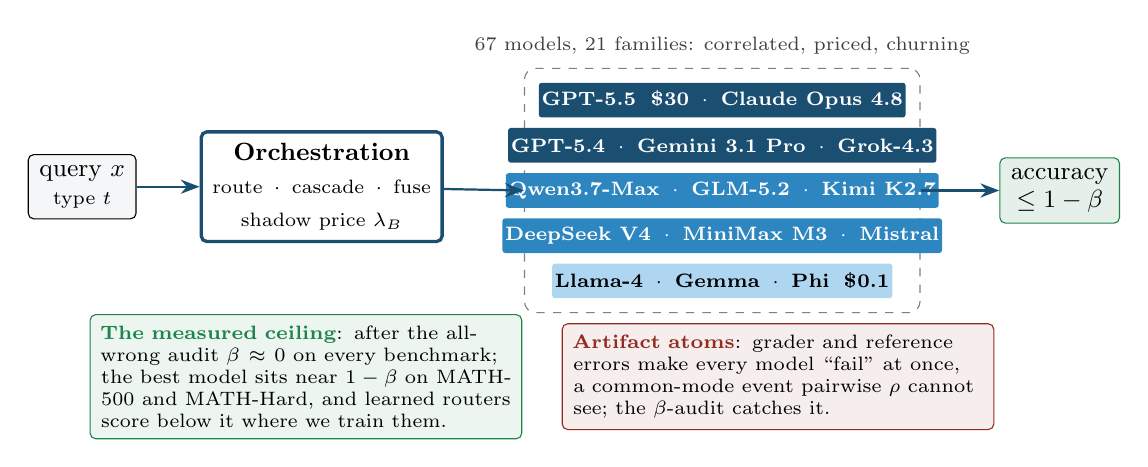
\begin{tikzpicture}[font=\small,
  box/.style={rounded corners=2pt, draw, align=center, inner sep=4pt},
  model/.style={rounded corners=1pt, draw=none, text=white, font=\scriptsize\bfseries, minimum width=30mm, minimum height=4.4mm, inner sep=1pt},
  arr/.style={-{Stealth[length=2.4mm]}, thick, draw=cfront}]
% query
\node[box, fill=cbg] (q) {query $x$\\[-1pt]\scriptsize type $t$};
% orchestration layer
\node[box, draw=cfront, very thick, fill=white, right=8mm of q, align=center] (orch)
  {\textbf{Orchestration}\\[1pt]\scriptsize route $\,\cdot\,$ cascade $\,\cdot\,$ fuse\\[1pt]\scriptsize shadow price $\lambda_B$};
% pool
\node[model, fill=cfront, right=12mm of orch, yshift=11mm] (m1) {GPT-5.5 \;\$30 \,$\cdot$\, Claude Opus 4.8};
\node[model, fill=cfront, below=1.2mm of m1] (m2) {GPT-5.4 \,$\cdot$\, Gemini 3.1 Pro \,$\cdot$\, Grok-4.3};
\node[model, fill=cmid, below=1.2mm of m2] (m3) {Qwen3.7-Max \,$\cdot$\, GLM-5.2 \,$\cdot$\, Kimi K2.7};
\node[model, fill=cmid, below=1.2mm of m3] (m4) {DeepSeek V4 \,$\cdot$\, MiniMax M3 \,$\cdot$\, Mistral};
\node[model, fill=ccheap, text=black, below=1.2mm of m4] (m5) {Llama-4 \,$\cdot$\, Gemma \,$\cdot$\, Phi \;\$0.1};
\begin{scope}[on background layer]
\node[draw=gray, dashed, rounded corners, fit=(m1)(m5), inner sep=5pt] (pool) {};
\end{scope}
\node[above=0.5mm of pool, font=\scriptsize, text=gray!50!black] {67 models, 21 families: correlated, priced, churning};
% output
\node[box, fill=cgain!12, draw=cgain, right=10mm of pool, align=center] (out) {accuracy\\[-1pt]$\le 1-\beta$};
\draw[arr] (q) -- (orch);
\draw[arr] (orch) -- (pool.west);
\draw[arr] (pool.east) -- (out);
% two-regime strip
\node[box, fill=cgain!8, draw=cgain, below=9mm of orch, xshift=-2mm, align=left, font=\scriptsize, text width=52mm] (r1)
  {\textbf{\textcolor{cgain}{The measured ceiling}}: after the all-wrong audit $\beta\approx0$ on every benchmark; the best model sits near $1-\beta$ on MATH-500 and MATH-Hard, and learned routers score below it where we train them.};
\node[box, fill=cceil!8, draw=cceil, right=5mm of r1, align=left, font=\scriptsize, text width=52mm] (r2)
  {\textbf{\textcolor{cceil}{Artifact atoms}}: grader and reference errors make every model ``fail'' at once, a common-mode event pairwise $\rho$ cannot see; the $\beta$-audit catches it.};
\end{tikzpicture}}
\caption{\label{fig:framework}\textbf{Orchestration is allocation.} A query is routed, cascaded, or fused over a priced,
correlated, fast-churning pool of $67$ frontier-to-cheap models; the optimal policy is a per-type bang-per-buck rule with a
single shadow price $\lambda_B$ on the inference dollar (Prop.~\ref{prop:duality}). No selection policy can exceed the ceiling
$1-\beta$ set by the rate $\beta$ at which \emph{all} models fail at once (Prop.~\ref{prop:cert}). The field reports pairwise
error correlation $\rho$ to decide whether to orchestrate; $\rho$ is blind to $\beta$, including to the spurious common-mode
failures that evaluation errors create.}
\end{figure}

\section{Related Work}\label{sec:related}
\paragraph{Routing and cascades.} Learned routers select one model per query \citep{ong2024routellm,ding2024hybridllm};
cascades escalate from cheap to strong on low confidence \citep{chen2023frugalgpt,madaan2023automix}.
\citet{dekoninck2024cascaderouting} unify the two and prove optimality of a routing strategy and an optimal cascade;
\citet{jitkrittum2023cascade} characterize the optimal two-model deferral rule and show confidence-based deferral can
be sub-optimal when the downstream model's errors are unmodeled, directly relevant to our calibration-and-edge
condition. \citet{hu2024routerbench} benchmark routing on pre-computed outcomes. These works treat the oracle as an
empirical ceiling and the cascade threshold as a tuned hyperparameter; we add the dollar stopping rule, the
calibration dominance boundary, and the volume ceiling they leave implicit.
\paragraph{Ensembling and fusion.} \citet{jiang2023llmblender} rank-and-fuse generations; \citet{wang2024moa} aggregate
in layers; \citet{li2024moreagents} sample-and-vote; \citet{li2025selfmoa} show that sampling the single best model
(Self-MoA) often beats heterogeneous fusion, attributing this to a quality--diversity trade-off (mixing helps only when
members are of similar quality). Classical ensemble theory supplies the variance decomposition
\citep{krogh1995ensemble,ueda1996}, its modern unification \citep{wood2023diversity}, and the caution that diversity does
not guarantee accuracy gains \citep{kuncheva2003}. The accuracy \emph{ceiling} we use is also classical: it is Kuncheva's
\emph{Oracle} combiner (correct iff some member is correct, i.e.\ $1-\beta$ \citep{kuncheva2004combining}) and the
majority-vote-accuracy limits of \citet{kuncheva2003limits}, both predating LLMs and presuming labels. Our contribution is
not the ceiling but (i) that it bounds \emph{every} selection policy, debate and self-consistency included, whose outputs
are a.s.\ member answers, and (ii) its conversion into a finite-sample \$0 \emph{certificate} (Prop.~\ref{prop:cert}) that
needs labels only on one graded held-out sample, and from it only the all-wrong count; an Oracle combiner needs the label of
every deployed query.
\paragraph{Error correlation and inference economics.} \citet{kim2025correlated} document, over $350+$ models, that
\emph{pairwise} errors are substantially correlated and rise with accuracy and shared provider, but they measure the
bivariate agree-when-wrong statistic on multiple-choice tasks and stop at qualitative implications; they neither define the
joint all-models-wrong rate $\beta$ nor bound any selection policy by it. We show that pairwise correlation provably cannot
identify $\beta$ for $m\ge3$ (Prop.~\ref{prop:nonid}), and that $\beta$, not $\rho$, is the ceiling. This monoculture of
errors traces to \citet{kleinberg2021monoculture}. Closest is \citet{turkmen2026ensembleselection}, who also fit a
tetrachoric Gaussian copula to binary LLM errors and derive an equicorrelated ensemble error \emph{floor}. We show that such a
floor underprices any common-mode atom, which a Gaussian copula cannot represent (zero lower tail dependence;
Prop.~\ref{prop:poolbias}). On the audited 2026 frontier we find no genuine atom on mathematics or science, but evaluation
errors produce one, and a pairwise-calibrated copula, Gaussian or Clayton, underprices it as predicted
(\S\ref{sec:results}). \citet{erol2025costofpass} formalize dollars-per-correct via production theory, our primary metric.
\paragraph{Finance and real options.} Mean--variance allocation \citep{markowitz1952}, cost-aware diversification
\citep{statman1987}, the value of information \citep{howard1966}, selective prediction \citep{geifman2017}, switching
costs \citep{klemperer1995}, and real-options volatility comparative statics \citep{mcdonald1986,dixit1994,merton1976}
are the antecedents we build on.

\section{Problem Formulation}\label{sec:setup-formal}
Queries $x$ carry a latent type $t=T(x)\sim D$, with type prior $p(t)=\Pr[T=t]$. A pool $M=\{1,\dots,m\}$ of models has
quality $q_i(t)\in[0,1]$ (expected per-query utility on type $t$) and price $c_i\ge 0$ (dollars/query); write
$\bar q_i=\E_t q_i(t)$. A (possibly stochastic) routing policy $\pi\colon T\to\Delta(M)$ has value
$V(\pi)=\E_t\sum_i \pi(i\mid t)\,q_i(t)$ and cost $K(\pi)=\E_t\sum_i \pi(i\mid t)\,c_i$. We also consider fusion (query
several, combine) and cascading (escalate on low confidence). The buyer's objective is dollars-per-correct
\citep{erol2025costofpass}, or quality subject to a budget; we make it explicit in each section.

\paragraph{Economic scaffolding (deferred to App.~\ref{app:econ}).} Treating orchestration as allocation yields a
compact economic layer that we use but do not foreground; the tools are standard and the empirical results below do
not depend on it. Three facts, stated and proved in App.~\ref{app:econ}: under a dollar budget, routing is a priced
assignment with a single shadow price $\lambda_B$ (Prop.~\ref{prop:duality}); cost-aware fusion has a diversification
limit $k^\ast(\rho,c)$ that shrinks as error correlation rises (Props.~\ref{prop:keven},~\ref{prop:lambda}), above the
classical equicorrelated variance floor (Prop.~\ref{prop:floor}); and a calibrated cascade collapses to
random mixing exactly as the verifier AUC falls to $1/2$, with a price-independent escalation ceiling $1-a_L/a_H$
(Prop.~\ref{prop:cascade}, Cor.~\ref{cor:edge}).

\section{Experimental Setup}\label{sec:setup}
We ran the pillar experiments on a pool of 15 current models across 9 provider families: frontier (Claude
Opus~4.8, GPT-5.1, Gemini~3.1~Pro, Kimi~K2.7), mid (Claude Sonnet~4.6, GPT-5-mini, Gemini~3.5~Flash, Qwen3-235B, Mistral-Large,
MiniMax~M2.7, DeepSeek~V3.2), and cheap (Claude Haiku~4.5, GPT-5-nano, Gemini~3.1~Flash-Lite, Llama-4-Maverick); exact dated
snapshots and prices are frozen in the registry (App.~\ref{app:repro}). The pillar experiments use five benchmarks: a saturated
mix (GSM8K, MMLU, ARC-Challenge, MATH-500; $120$ queries each) and a harder set (MMLU-Pro; $200$ queries). For the
\emph{market-scale} realizability measurement (\S\ref{sec:realiz}) we expand the pool to $67$ models across $21$ provider
families---the live OpenRouter catalog from the current frontier down to small open-weights (GLM, Qwen, DeepSeek, MiniMax,
Nemotron, Llama-3.x, Mistral, Gemma, Phi, Granite, and others), chat/instruct only, with live-verified prices (full named roster, App.~\ref{app:roster})---and add hard domains that probe co-failure: open-ended competition
mathematics on three benchmarks (MATH-500, MATH Level-5 ``MATH-Hard'', and AIME-2024/2025, whose integer answers leave no
room for formatting disputes and whose release post-dates the older models' training cutoff) and graduate-level science (GPQA-Diamond, Physics/Chemistry/Biology). Mathematics, AIME, GSM8K and code prompts ask the model to reason and then answer, and GPQA asks for a boxed letter; MMLU,
ARC and MMLU-Pro ask for the answer letter only, a direct-answer protocol that lowers accuracy for models that obey it (the
exact prompts are in \texttt{items\_snapshot.json}). Grading is programmatic for all of these benchmarks
(\texttt{harness/grade.py}): numeric answers, multiple-choice letters, and mathematical answers compared after the MATH
benchmark's reference answer normalization (units, thin spaces, equivalent fraction forms, $\pm$, unordered answer lists)
with a symbolic-equivalence fallback, so no LLM judge is used there; the first release's grader lacked that normalization
(App.~\ref{app:audit}). The one exception is the content-controlled free-response GPQA test (App.~\ref{app:opengpqa}), graded
by a five-judge LLM panel. Every question on which all models are graded wrong is audited before it counts toward $\beta$
(\S\ref{sec:results}).
Costs are the list-price costs logged with every call (OpenRouter is an aggregator, so this is not per-provider
reconciliation). The core pillar experiments cost \$\nCostCore{} and the market-scale measurement \$\nCostMarket{} (itemized in
\texttt{cost\_registry.csv}); the execution-graded code run's logged per-cell costs sum to \$\nCostCode. Every call of the project
that returned a response, including exploratory and superseded runs, is listed in \texttt{spend\_ledger.csv}: \$\nSpendJune{} over
$\nCallsJune$ calls in June 2026, and \$\nSpendAudit{} for this version's audit (App.~\ref{app:audit}). Baselines: single-cheapest,
single-best (selected in-sample for the ceiling measurements, which can only overstate $a_{\mathrm{sb}}$ and so understate
$G=V^o-a_{\mathrm{sb}}$; the certificate therefore replaces $a_{\mathrm{sb}}$ by its Bonferroni lower confidence limit over
models, and every router comparison selects the single best model on a training split), random and random-mixing-at-matched-budget, cost-matched
Self-MoA \citep{li2025selfmoa}, a partition-conditioned oracle and a partition-free per-query oracle, a confidence cascade,
majority vote, and heterogeneous fusion.

\section{Results}\label{sec:results}
All correctness is re-scored from the logged model responses by the corrected grader of \S\ref{sec:setup}
(\texttt{harness/grade.py}); the first release scored several matrices with earlier extractors whose defects are listed in
App.~\ref{app:audit}.

\begin{table}[h]\centering\small
\begin{tabular}{lcc}
\toprule
Quantity & Saturated multi-domain mix & Hard single-domain (MMLU-Pro) \\
\midrule
Single-best & \nTaMixSB{} (\nTaMixSBName) & \nTaProSB{} (\nTaProSBName) \\
Oracle (per-query) & \nTaMixOracle & \nTaProOracle \\
\textbf{Oracle gain $G$ (95\% CI)} & \textbf{\nTaMixG} $[\nTaMixGLo,\nTaMixGHi]$ & \textbf{\nTaProG} $[\nTaProGLo,\nTaProGHi]$ \\
mean off-diagonal $\rho$ & \nTaMixRho & \nTaProRho \\
within-family $\rho$ & \textbf{\nTaMixRhoIn} & \textbf{\nTaProRhoIn} \\
cross-family $\rho$ & \nTaMixRhoX & \nTaProRhoX \\
\bottomrule
\end{tabular}
\caption{Pillar A in two regimes (re-graded; $G$ with $2000$-resample query-bootstrap 95\% CIs, $N{=}\nTaMixN$ and $\nTaProN$). $G>0$ with
both CIs excluding zero confirms $Q$ is not row-dominated (Lem.~\ref{lem:env}), and the point estimate of $G$ is larger on the harder, more
dispersed regime (the CIs overlap). Within-family $\rho$ exceeds cross-family on the multi-domain mix (gap $\nTaMixRhoGap$) but not on MMLU-Pro
($\nTaProRhoGap$): family specialization shows across domains rather than within one, consistent with the shared-provider
correlation of \citet{kim2025correlated}.}\label{tab:A}
\end{table}

\paragraph{Pillar A: the oracle gain is real, and no router realizes it.} Oracle gain $G>0$ with bootstrap CIs excluding zero in
both regimes ($\nTaMixG$ saturated, $\nTaProG$ hard; Table~\ref{tab:A}): a per-query oracle would help, \emph{modestly because
the frontier agrees}, and
(in point estimate; the CIs overlap) more on the harder, more dispersed regime, the dispersion signature the theory predicts. Within-family $\rho$ exceeds cross-family on
the multi-domain mix but not on the single-domain set. The cost--quality frontier is populated by cheap models
(Fig.~\ref{fig:cq}). No router we train beats the single best model, and the learned ones fall below it. On held-out
queries, with the single best model chosen on the training split, a TF-IDF$+$domain logistic router attains $\nRtLearned$
against single-best $\nRtSB$ on the mix: it captures $\nRtFrac$ of $G$ ($95\%$ CI $[\nRtFracLo,\nRtFracHi]$, excluding
zero), losing $\nRtLost$ of $\nRtN$ held-out queries, as many as a perfect router would gain. To rule out a weak-baseline artifact we tried three stronger
routers, and none beats the single best model. A gradient-boosted per-model correctness predictor on word$+$char TF-IDF features captures
$\nRtGbm$ of $G$, and a direct multiclass best-model predictor $\nRtMulti$. A deployment-realistic \emph{LLM-as-router}
(GPT-5-mini shown each query and a capsule of every model's strengths, asked to pick the best) routes to single-best on
$\nRtLlmRoutePct\%$ of queries and so captures exactly $\nRtLlmFrac$ of $G$ (\texttt{router\_strong.py},
\texttt{router\_llm.py}). On the hard MMLU-Pro pool the learned router is also below single-best ($\nRtHardFrac$ of $G$, $\nRtHardLost$ of
$\nRtHardN$ held-out queries; not significant).
The routers are evaluated on the $15$-model pools, the pools on which we ran the router experiments; we did not train a router
on the market-scale ($\nMathM$-model) or GPQA matrices, so the market-scale routing statement rests on the certificate of
Prop.~\ref{prop:cert}, not an end-to-end
routing run. Against the
cost-aware oracle (optimal) frontier all sit far below the upper bound (Fig.~\ref{fig:router}). The realizable routing gain is thus
zero or negative. That four routers of increasing strength all fail suggests the prompt carries little signal about which
model will be right when the frontier disagrees, though with $G$ equal to $\nRtLost$ held-out queries we cannot rule out that a
stronger router would find some: the small oracle bound is itself largely unreachable.

\paragraph{Tail co-failure: a realizability certificate and its measurement.}\label{sec:realiz}
Why is the realizable gain near zero, and the oracle gain itself small? Both are governed by how often the pool fails
together. The next proposition makes the ceiling exact and turns it into a \$0 pre-deployment test; we then measure it on the
frontier.

\begin{proposition}[Ceiling, gain localization, and a realizability certificate]\label{prop:cert}
Let $\beta=\Pr_t[\text{all } m \text{ wrong}]$, $a_{\mathrm{sb}}=\max_i\bar q_i$, and $i^\star=\arg\max_i\bar q_i$.
\emph{(i)~Ceiling.} Any selection policy---a router, a (weighted) vote, or a cascade, whose output is almost surely one of
the members' answers---has accuracy at most $1-\beta$, attained by the per-query oracle, so the maximum gain over single-best
is exactly $\Delta^{\mathrm{ceil}}=(1-\beta)-a_{\mathrm{sb}}$. \emph{(ii)~Gain localization.} $G=V^o-a_{\mathrm{sb}}=\Pr_t[\text{single-best wrong}]-\beta$,
supported entirely on the \emph{resolvable} mass (non-unanimous, single-best wrong); the co-failure tail $\beta$ contributes
nothing to $G$. \emph{(iii)~Certificate.} From $n$ i.i.d.\ queries with $K$ all-wrong, let $\beta_{\mathrm{lo}}(K,n,\delta)$ be
the one-sided Clopper--Pearson lower confidence limit at level $1-\delta$; then with probability $\ge1-\delta$ every selection policy obeys
$\mathrm{Acc}-a_{\mathrm{sb}}\le(1-\beta_{\mathrm{lo}})-a_{\mathrm{sb}}$. If this certified bound falls below the orchestration
overhead, no policy in the class can pay for itself---a \$0 test ($a_{\mathrm{sb}}$ replaceable by its own \emph{lower} confidence bound).
\end{proposition}
\noindent Parts~(i)--(ii) are elementary identities, with one-line proofs (App.~\ref{app:proofs}): on the all-wrong event every member is wrong, so any selector is wrong;
and $G$ rearranges $V^o=1-\beta$. Their force is in use: part~(iii) turns them into a pre-deployment \$0
instrument, and part~(ii) corrects a tempting misstatement: a \emph{small} $\beta$ does not by itself imply orchestration cannot
help; it implies a high ceiling. The binding quantity is $\Delta^{\mathrm{ceil}}=(1-\beta)-a_{\mathrm{sb}}$, which is small on
the frontier only because $a_{\mathrm{sb}}$ already sits near the ceiling; the certificate is most informative exactly there.


\paragraph{The certified ceiling on the 2026 frontier.} Table~\ref{tab:cert} applies the certificate to every benchmark. On
MATH-500, MATH-Hard, AIME and multiple-choice GPQA-Diamond, no question defeats every model once the all-wrong questions are
audited (below): $\beta=0$, with a $95\%$ Clopper--Pearson upper limit of $\nMathBetaHi$ on MATH-500 ($n{=}\nMathN$) and
$\nHardBetaHi$ on MATH-Hard ($n{=}\nHardN$). $\beta$ is measured on the questions every model answered, and none of the
questions left out is failed by every model that answered it ($\nTotPartK$ such questions): the one candidate, an AIME-2025
question answered by 51 of 52 models, 30 of them at the token budget, is solved by six models when re-asked with $32{,}768$
tokens. The ceiling $1-\beta$ is therefore effectively $1$, and the operative question is
how close the best single model already sits. On MATH-500 and MATH-Hard it sits very close---$\nMathSB$ (\nMathSBName) on MATH-500 and
$\nHardSB$ on MATH-Hard---so the certified largest gain any router, vote or cascade could deliver over it is at most
$\nMathCert$ and $\nHardCert$ ($95\%$ confidence, with $a_{\mathrm{sb}}$ replaced by its Bonferroni lower limit over models).
Where the best model is weaker there is headroom: AIME ($G=\nAimeG$) and GPQA ($G=\nGmcG$). By Prop.~\ref{prop:cert}(ii) that
headroom is resolvable disagreement, not co-failure, and realizing it requires knowing, per query, which model to trust---the
signal the routers above could not find. Genuine co-failures appear only on MMLU-Pro, asked for a direct answer:
$\nMmluK$ of $\nMmluN$ across all $\nMmluM$ models and $\nProK$ of $\nProN$ in the 15-model pool ($\nGenuineQ$ distinct
questions); the saturated mix has $\nMixK$ of $\nMixN$. Both raters found both questions to admit more than one defensible answer, so this is an upper bound. On the
67-model question the single-factor model predicts $\nMmluRatioTet\times$ fewer all-wrong questions than observed: one
question, but the direction Prop.~\ref{prop:poolbias} predicts. On code, graded with special checkers wherever a problem accepts several correct outputs, none of the $\nCodeN$
problems defeats every model ($95\%$ upper limit $\nCodeBetaHi$).

\begin{table}[h]\centering\small\setlength{\tabcolsep}{3.2pt}
\begin{tabular}{lcccccccc}
\toprule
benchmark & \shortstack{models /\\queries} & \shortstack{single\\best} & oracle & $G$ & \shortstack{all-wrong\\(graded)} & genuine & \shortstack{$\beta$ 95\%\\upper} & \shortstack{certified\\max gain} \\
\midrule
MATH-500 & \nMathM{} / \nMathN & \nMathSB & \nMathOracle & \nMathG & \nMathAwGraded & \nMathK & \nMathBetaHi & \nMathCert \\
MATH-Hard & \nHardM{} / \nHardN & \nHardSB & \nHardOracle & \nHardG & \nHardAwGraded & \nHardK & \nHardBetaHi & \nHardCert \\
AIME 2024+25 & \nAimeM{} / \nAimeN & \nAimeSB & \nAimeOracle & \nAimeG & \nAimeAwGraded & \nAimeK & \nAimeBetaHi & \nAimeCert \\
GPQA-Diamond (MC) & \nGmcM{} / \nGmcN & \nGmcSB & \nGmcOracle & \nGmcG & \nGmcAwGraded & \nGmcK & \nGmcBetaHi & \nGmcCert \\
MMLU-Pro & \nMmluM{} / \nMmluN & \nMmluSB & \nMmluOracle & \nMmluG & \nMmluAwGraded & \nMmluK & \nMmluBetaHi & \nMmluCert \\
code\_contests$^{\dagger}$ & \nCodeM{} / \nCodeN & \nCodeSB & \nCodeOracle & \nCodeG & \nCodeAwGraded & \nCodeK & \nCodeBetaHi & \nCodeCert \\
15-model mix & \nMixM{} / \nMixN & \nMixSB & \nMixOracle & \nMixG & \nMixAwGraded & \nMixK & \nMixBetaHi & \nMixCert \\
15-model MMLU-Pro & \nProM{} / \nProN & \nProSB & \nProOracle & \nProG & \nProAwGraded & \nProK & \nProBetaHi & \nProCert \\
\bottomrule
\end{tabular}
\caption{The certified ceiling per benchmark (\texttt{canonical.py}). ``All-wrong (graded)'': questions every model fails under
the corrected grader; ``genuine'': those that survive the audit (reference errors and ambiguous questions removed); $\beta$ upper: two-sided $95\%$ Clopper--Pearson limit on the genuine rate; certified max gain: the
Prop.~\ref{prop:cert}(iii) upper bound on the gain of any selection policy over the single best model ($\delta=0.05$).
$^{\dagger}$Problems that accept several correct outputs are graded with special checkers where exact match would decide an
all-wrong question (App.~\ref{app:codegen}).}\label{tab:cert}
\end{table}

\paragraph{The all-wrong audit.} Our first release reported a co-failure tail on MATH-500 ($\nMathJuneK/\nMathJuneN$), MATH-Hard
($\nHardJuneK/\nHardJuneN$) and code ($\nCodeJuneK/\nCodeJuneN$). Table~\ref{tab:trace} traces every one of its $\nTotJune$ all-wrong events ($\nTotJuneQ$ distinct questions; a question in two pools counts once
per pool) through four checks, applied in
order: responses that were corrupt (no usage record, empty or cut-off content) were re-queried; answers that hit their token
budget were re-asked with $32{,}768$ tokens; the corrected grader re-scored every response; and each question still failed by
every model was adjudicated by two AI raters who solved it blind to the reference answer and to every model output, under a
classification rule written before the second rater's labels were read (App.~\ref{app:audit}). Each event is attributed to
the first check that removes it (in the 15-model pools the longer budget came after re-grading). $\nTotGrader$ were grader
defects---reference answers no response could match as written (``$x{=}5$'' against $5$, ``$10{,}\!080$'' against $10080$,
``$864\ \mathrm{inches}^2$'' against $864$) multiple-choice letters the extractor missed, or valid alternative outputs to code problems that exact-match
grading rejected; $\nTotRefErr$ were wrong reference
answers (the arithmetic-series question in MATH-Hard, whose reference $3$ should be $-3$, is one); $\nTotAmbig$ were ambiguous
questions; $\nTotTrunc$ were resolved by the longer budget; $\nTotCorrupt$ by
re-querying a corrupt response; and $\nTotGenuine$ were genuine, on $\nTotGenuineQ$ distinct MMLU-Pro questions. The first release's free-response GPQA tail ($\nOpenOneK$
questions) was likewise $\nOpenOneOpt$ questions that depend on stripped options and $\nOpenOneDoubt$ with doubtful references
(App.~\ref{app:opengpqa}).

\begin{table}[h]\centering\small\setlength{\tabcolsep}{3.4pt}
\begin{tabular}{lccccccc}
\toprule
 & \shortstack{June\\all-wrong} & corrupt & \shortstack{trun-\\cation} & grader & \shortstack{wrong\\ref.} & \shortstack{ambi-\\guous} & genuine \\
\midrule
MATH-500 (67) & \nMathJuneK & \nMathJuneCorrupt & \nMathJuneTrunc & \nMathJuneGrader & \nMathJuneRefErr & \nMathJuneAmbig & \nMathJuneGenuine \\
MATH-Hard (67) & \nHardJuneK & \nHardJuneCorrupt & \nHardJuneTrunc & \nHardJuneGrader & \nHardJuneRefErr & \nHardJuneAmbig & \nHardJuneGenuine \\
code\_contests (18) & \nCodeJuneK & \nCodeJuneCorrupt & \nCodeJuneTrunc & \nCodeJuneGrader & \nCodeJuneRefErr & \nCodeJuneAmbig & \nCodeJuneGenuine \\
MMLU-Pro (67) & \nMmluJuneK & \nMmluJuneCorrupt & \nMmluJuneTrunc & \nMmluJuneGrader & \nMmluJuneRefErr & \nMmluJuneAmbig & \nMmluJuneGenuine \\
GPQA-Diamond MC (52) & \nGmcJuneK & \nGmcJuneCorrupt & \nGmcJuneTrunc & \nGmcJuneGrader & \nGmcJuneRefErr & \nGmcJuneAmbig & \nGmcJuneGenuine \\
15-model mix & \nMixJuneK & \nMixJuneCorrupt & \nMixJuneTrunc & \nMixJuneGrader & \nMixJuneRefErr & \nMixJuneAmbig & \nMixJuneGenuine \\
15-model MMLU-Pro & \nProJuneK & \nProJuneCorrupt & \nProJuneTrunc & \nProJuneGrader & \nProJuneRefErr & \nProJuneAmbig & \nProJuneGenuine \\
\midrule
total & \nTotJune & \nTotCorrupt & \nTotTrunc & \nTotGrader & \nTotRefErr & \nTotAmbig & \nTotGenuine \\
\bottomrule
\end{tabular}
\caption{Every all-wrong question of the June 2026 release, by the first check that removes it (\texttt{canonical.py},
\texttt{rerun\_log.csv}, \texttt{audit/adjudication\_result.json}). A question counts as genuine only if it survives all four.}\label{tab:trace}
\end{table}

\paragraph{What pairwise $\rho$ saw: an artifact atom.} The spurious MATH-500 tail is instructive, because it is a genuine
common-mode atom---not of model failure but of evaluation failure: a reference answer that no response can match makes every
model wrong at once, however diverse the models are. Analysed exactly as our first release analysed it, it has every signature
of the co-failure the paper's theory describes. Its $\nArtK$ all-wrong questions (the June tail after the truncation control; $\beta=\nArtBeta$ over $n{=}\nArtN$) are
$\nArtRatioTet\times$ the rate a tetrachoric-calibrated single-factor model predicts from the pairwise correlations
($\bar\rho_{\mathrm{tet}}=\nArtRhoTet$, $\beta_{\mathrm{sf}}=\nArtBsfTet$; bootstrap $90\%$ interval $\nArtRatioLo$--$\nArtRatioHi$),
$\nArtFullRatio\times$ what the full pairwise Gaussian copula predicts, and $\nArtClayRatio\times$ what a lower-tail-dependent
Clayton copula ($\lambda_L=\nArtClayLam$) predicts; and the ratio grows with pool size, from $\nArtCompStart$ at $k{=}2$ to
$\nArtCompEnd$ at $k{=}\nArtM$ (Fig.~\ref{fig:realizability}). Our first release read that signature as frontier co-failure.
It was the grader. The lesson generalizes: the underpricing signature is what a \emph{common mode} produces (though smooth
tail dependence can also make it grow at finite pool size; see the Clayton control below), it says nothing about the cause, and
the cheapest common mode to create is an evaluation error. Pairwise statistics cannot distinguish the two; reading the
all-wrong questions can.

\begin{figure}[tbp]\centering
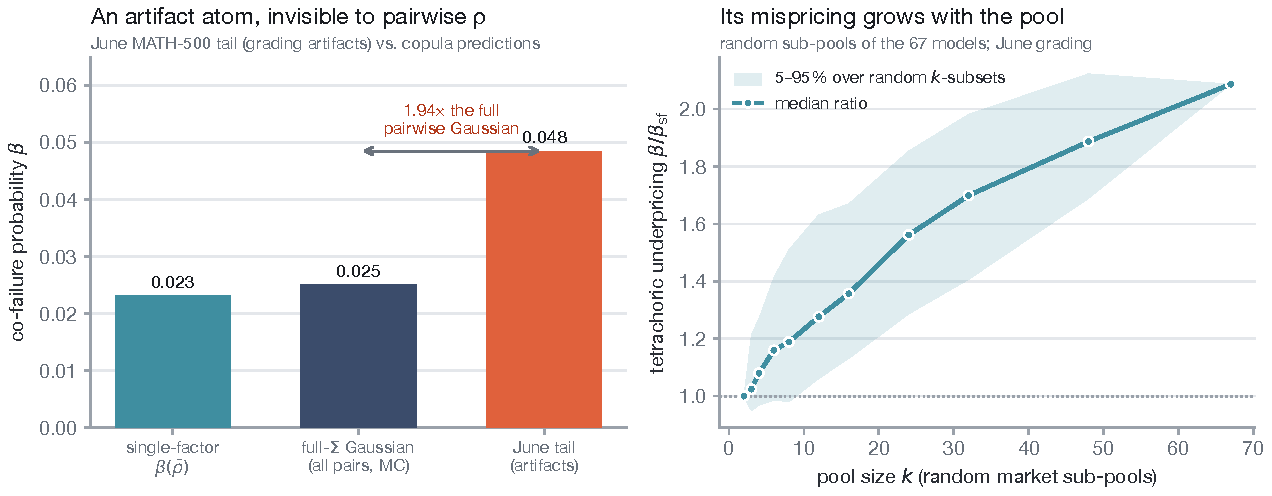
\includegraphics[width=0.92\textwidth]{figures/fig_realizability.pdf}
\caption{\label{fig:realizability}An evaluation-error atom, as a pairwise model sees it (the June MATH-500 tail, $\nArtM$ models,
$\nArtK$/$\nArtN$ questions, every one a grading artifact; App.~\ref{app:audit}). \emph{Left}: the single-factor tetrachoric
copula ($\beta(\bar\rho)=\nArtBsfTet$) and the full pairwise-tetrachoric Gaussian copula ($\nArtFullBeta$) both predict far fewer
all-wrong questions than the artifact produces ($\nArtBeta$). \emph{Right}: over random $k$-model sub-pools ($\nArtCompPools$ per
size; band $5$--$95\%$), the underpricing grows with pool size, the signature Prop.~\ref{prop:poolbias} proves for any common-mode
atom. Computed by \texttt{canonical.py}.}
\end{figure}

Growth of this kind is forced by any common-mode atom, which we now prove; growth alone does not prove an atom, since a
Clayton copula without one also grows at finite pool size (below).

\begin{proposition}[Pairwise $\rho$ underprices co-failure, with bias growing in pool size]\label{prop:poolbias}
Model errors by a common-shock mixture: each query is \emph{co-hard} with probability $\omega\in(0,1)$ (all $m$ models err
together) and otherwise each model errs independently with probability $\alpha_0\in(0,1)$. The marginal error rate is
$\alpha=\omega+(1-\omega)\alpha_0$ and the pairwise error correlation is
$\bar\rho=[\omega+(1-\omega)\alpha_0^2-\alpha^2]/[\alpha(1-\alpha)]>0$. The true co-failure rate is
$\beta(m)=\omega+(1-\omega)\alpha_0^{\,m}$. Let $\beta_{\mathrm{sf}}(m)$ be the all-wrong rate of the single-factor Gaussian copula
calibrated to $(\alpha,\bar\rho)$, i.e.\ with the latent (tetrachoric) correlation $\rho_{\mathrm{tet}}\in(0,1)$ that reproduces the
pairwise co-error $\omega+(1-\omega)\alpha_0^2$. Then (i) $\beta(m)\downarrow\omega>0$ while $\beta_{\mathrm{sf}}(m)\downarrow0$, because a Gaussian
copula with $\rho_{\mathrm{tet}}<1$ has zero lower tail dependence \citep{sibuya1959bivariate,embrechts2002correlation}; hence (ii) the underpricing ratio
$\beta(m)/\beta_{\mathrm{sf}}(m)\to\infty$ and is eventually strictly increasing in $m$, while equalling $1$ at $m=2$. In this
exchangeable model, $\alpha$ and the mean pairwise $\rho$ fix the \emph{bivariate} error law but discard the higher-order dependence that
governs joint failure of a large pool; they are exact for pairs and increasingly inadequate as the pool grows.
\end{proposition}
\noindent The classical ingredient---a Gaussian/elliptical copula has zero lower tail dependence
\citep{sibuya1959bivariate}, so a common-mode atom (Marshall--Olkin-type shared-failure component;
\citealp{marshall1967multivariate}) cannot be represented by any pairwise calibration---is not ours; the body--vs--tail
underpricing it implies is the base-correlation ``smile'' familiar from Gaussian-copula credit models
\citep{li2000default,donnelly2010devil}. New here is the \emph{transfer} to LLM orchestration: the co-failure
instantiation, the pool-size-divergence framing, and a real instance. The evaluation-error atom of our first release
(Fig.~\ref{fig:realizability}) has the monotone shape this predicts: ratio $\approx1$ at $k{=}2$, growing with
$k$. The exchangeable, homogeneous model licenses the mechanism and the sign---any common-mode atom ($\beta_\infty>0$) forces the
divergence---while the heterogeneous magnitude (the $\nArtCompStart\times\!\to\!\nArtCompEnd\times$ curve on that tail) is
empirical. It also says precisely \emph{why} a buyer cannot price orchestration from the reported statistic:
$\rho$ certifies pairwise substitutability, not the tail in which orchestration either pays or does not.

\noindent\textbf{The driver is a common mode, not tail dependence \emph{per se}.} It is tempting to attribute the effect to
the lower tail-dependence coefficient $\lambda_L$, but that is false, and the distinction is the substance of the result. What
pairwise $\rho$ misses is a \emph{common-mode atom}: a positive-probability event of joint failure, $\beta_\infty:=\lim_m\beta(m)>0$,
that the pairwise correlation underweights. Smooth tail dependence that is \emph{already reflected} in $\rho$ does not produce the
effect. We verified the dichotomy in a logged simulation (\texttt{copula\_dichotomy.py}; it uses the Pearson-of-indicators
calibration, so absolute ratios are inflated and only the contrast is meaningful): an exchangeable
Clayton copula (Archimedean, $\lambda_L=2^{-1/\theta}$) yields only \emph{modest}, slowly growing underpricing under the same
binary-$\rho$ pipeline---$\nDiRatioA\times$ at $m{=}\nDiM$ for $\lambda_L{=}\nDiLamA$, and \emph{smaller} ($\nDiRatioB\times$) for larger
$\lambda_L{=}\nDiLamB$, because higher $\lambda_L$ raises the pairwise $\rho$ the single-factor model then absorbs. (Its all-wrong
rate still vanishes, like $m^{-1/\theta}$, so the ratio grows at most polynomially and is damped by tail dependence.) A
common-shock mixture with the same marginals but a rare shared-failure atom ($\beta_\infty{=}0.05$; its pairwise
$\bar\rho$ is $\nDiRhoAtom$ against $\nDiRhoA$ for the first Clayton case, so the contrast is between mechanisms, not at matched
correlation) instead drives the ratio past
$10^{\nDiAtomExp}\times$. The
orchestration-relevant object is thus the multivariate co-failure floor $\beta_\infty$, which no single pairwise number can
identify; this both sharpens the certificate of Prop.~\ref{prop:cert} and explains why the gap \emph{widens} with pool size
(pairwise $\rho$ saturates while $\beta_\infty$ does not). We state the underlying non-identification exactly.

\begin{proposition}[Non-identification of the co-failure floor; specialization of a classical Fr\'echet-class fact]\label{prop:nonid}
For $m\ge3$ the co-failure rate $\beta=\Pr[\text{all }m\text{ wrong}]$ is \emph{not} a function of the pairwise error law:
there exist joint distributions over $\{0,1\}^m$ with identical one- and two-dimensional marginals---hence identical marginal
error rates and identical pairwise correlations, Pearson \emph{and} tetrachoric---yet different $\beta$. Consequently no
statistic computed from pairwise correlations, a single-factor copula included, can identify $\beta$ or the large-pool floor
$\beta_\infty$; the common-shock atom and a matched-$\bar\rho$ Gaussian dependence (Prop.~\ref{prop:poolbias}) are precisely the
two extremes of this ambiguity ($\beta_\infty>0$ versus $\beta_\infty=0$ at identical pairwise law).
\end{proposition}
\noindent The mathematics is classical: the proof (App.~\ref{app:proofs}) is the fact that low-order
marginals underdetermine a joint on $\{0,1\}^m$ for $m\ge3$ (the Fr\'echet class has positive dimension;
\citealp{fontana2018representation}), instantiated for the co-failure cell. The consequence for practice is that pairwise $\rho$ cannot, even in principle, see the
quantity that caps orchestration, so a direct estimate of $\beta$ (with the certificate of Prop.~\ref{prop:cert}), not any function of $\rho$, is
the right instrument.


\paragraph{Graduate science in both answer formats: a content-controlled test.} We re-asked the same GPQA-Diamond
questions as free response, graded by a five-judge LLM panel (pairwise $\kappa=\nKappaLo$--$\nKappaHi$; App.~\ref{app:opengpqa}).
Removing the options leaves some questions unanswerable (``which statement below\ldots''), so all $130$ were screened under a
protocol fixed before any new data were collected, by raters who never saw a model answer: $80$ are kept as written, $5$ are
rewritten to ask for the same answer without the options, and $45$ are excluded because the question depends on its options
($22$) or the reference answer is not a unique free-response answer ($23$). On the $\nOpenN$ well-posed questions that every
model answered, \textbf{no co-failure tail opens}: $\beta=\nOpenBeta$ ($\nOpenK$ of $\nOpenN$; $95\%$ upper bound
$\nOpenBetaHi$), as in multiple choice on the same questions ($\nOpenMcK$ of $\nOpenMcN$). Counting the partially answered
questions on which every answering model missed as co-failures gives at most $\nOpenUpK$ of $\nOpenUpN$. Accuracy changes little
with the format (on the $\nOpenMatchModels$ models in both runs, mean $\nOpenMcMean\!\to\!\nOpenOpenMean$, best
$\nOpenMcBest\!\to\!\nOpenOpenBest$), and the models miss different questions. The secondary analysis specified in the protocol, which also
keeps the $23$ questions with a doubtful reference answer, finds $\nOpenSecK$ all-wrong questions of $\nOpenSecN$, and all
$\nOpenSecFlagged$ are among those $23$. \textbf{This retracts a claim of our first version}, which reported $\beta=\nOpenOneBeta$ on
free-response GPQA and read it as evidence that answer format, not content, sets the regime; that estimate came from
option-dependent questions and a judge that saw only the first 2{,}000 characters of each answer (App.~\ref{app:audit}). On the primary question set, graduate-level science is realizability-bound in both formats, like every other benchmark we
test; the secondary set's $\nOpenSecK$ all-wrong questions ($95\%$ CI on $\beta$ $[\nOpenSecBetaLo,\nOpenSecBetaHi]$) all
have a doubtful reference.

\begin{figure}[t]\centering
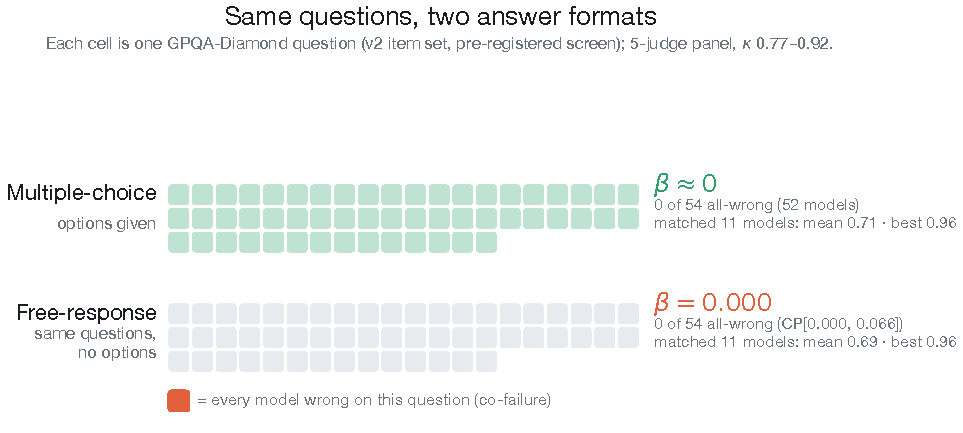
\includegraphics[width=0.94\textwidth]{figures/fig_format_flip.pdf}
\caption{\label{fig:flip}\textbf{Same questions, two answer formats.} The $\nOpenN$ well-posed GPQA-Diamond questions that
every model answered (protocol screen, App.~\ref{app:opengpqa}), asked as multiple choice (top) and as free response
(bottom; five-judge panel, $\kappa$ $\nKappaLo$--$\nKappaHi$). Each cell is one question; an orange cell would mark a question
on which \emph{every} model is wrong. Neither format has one ($\nOpenMcK$ and $\nOpenK$). Recomputed from \texttt{runs/canonical.json}.}
\end{figure}

\begin{figure}[t]\centering
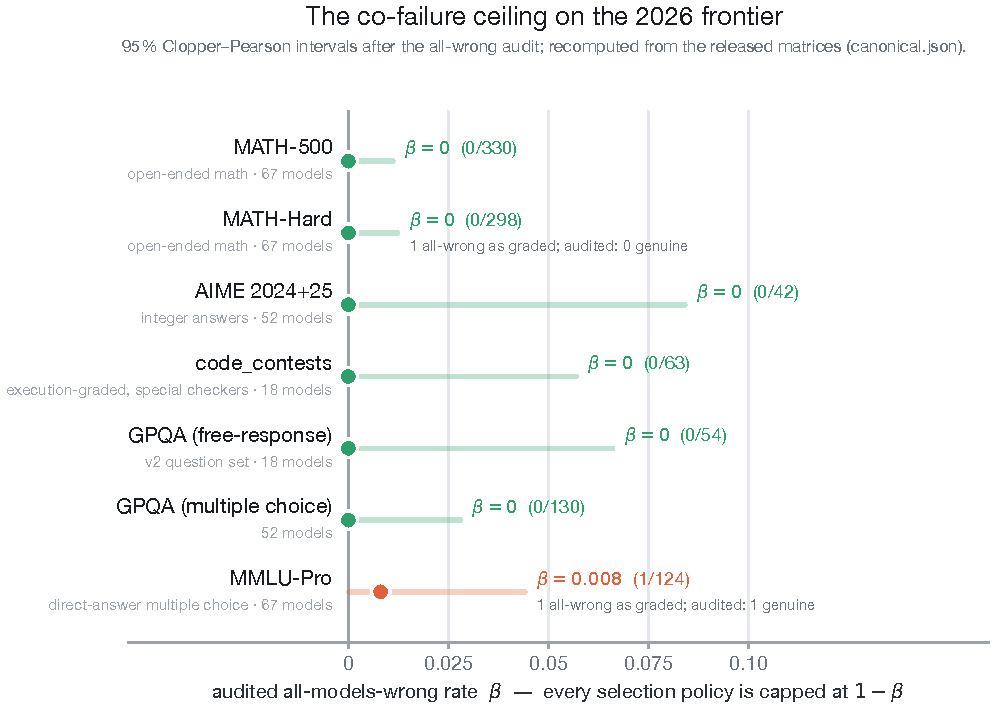
\includegraphics[width=0.97\textwidth]{figures/fig_regime_map.pdf}
\caption{\label{fig:regimemap}\textbf{The co-failure ceiling on the 2026 frontier.} Audited all-models-wrong rate $\beta$ per
benchmark with $95\%$ Clopper--Pearson intervals, and the as-graded count before the audit. Every benchmark is
realizability-bound: $\beta$ is zero or near zero, so the oracle gain is resolvable disagreement that a router would have to
capture. Recomputed from the released matrices by \texttt{canonical.py}.}
\end{figure}

\paragraph{Pillar B: voting loses, and diversity does not rescue it.} \emph{(1) Naive diversity is a
liability.} On all $\binom{15}{3}=455$ three-model triplets, regressing the unweighted majority-vote gain over the best member
on $\rho$ with accuracy-headroom control and model-clustered (leave-one-model-out jackknife) inference, the mean vote gain is
negative ($\nBGainHard$ hard, $\nBGainSat$ saturated). It stays negative whichever model is dropped (at most
$\nBGainLooHardMax$ and $\nBGainLooSatMax$), and the vote loses to its own best member on $\nBNegHardPct\%$ and
$\nBNegSatPct\%$ of triplets: mixing unequal-quality models lets diverse-but-weaker members outvote a strong one. The finer
prediction that the gain rises as $\rho$ falls is not supported: the slope on $\rho$ is $\nBSlope$ (hard pool), the opposite
sign, and not significant under model-clustering (jackknife 95\% CI $[\nBSlopeLo,\nBSlopeHi]$; the naive i.i.d.\ bootstrap CI
is $\approx\!\nBWidthRatio\times$ too narrow; Fig.~\ref{fig:rho}). Voting over a diverse pool thus loses to its own best member,
consistent with \citet{li2025selfmoa,kuncheva2003}. \emph{(2) Even at matched quality,
diversity buys little.} We test the diversification theorem in its most favourable regime by contrasting Self-MoA (distinct
samples of the single best model; high intra-model error correlation $\rho{=}\nEqRhoSelf$) against heterogeneous fusion over an
6-model band of similar accuracy (members $\nEqMemLo$--$\nEqMemHi$; lower inter-model correlation $\rho{=}\nEqRhoHet$, estimated on
a disjoint sample split), with $S{=}9$ so Self-MoA scales on distinct draws rather than recycling a fixed budget
(Fig.~\ref{fig:eqq}). At the \emph{information-fair} comparison ($k{=}3$, equal distinct draws per side) the heterogeneous
ensemble is ahead by $\nEqKThree$ (query-bootstrap CI $[\nEqKThreeLo,\nEqKThreeHi]$). Across $\nEqTrials$ resamplings of the
sample-to-split partition the gain averages $\nEqMean$ (range $\nEqMin$ to $\nEqMax$; positive in $\nEqPosPct\%$ of them), and an
alternative aggregation gives $\nEqAltAgg$. Over $k=1,\dots,\nEqKMax$ the largest gain is $\nEqBestDiff$ (at $k{=}\nEqBestK$), and
the CI excludes zero only at $k{=}\nEqSigK$. Under the primary (distinct-draw) aggregation the sign the diversification limit predicts appears on average; under the alternative
aggregation (\texttt{fusion.py}, whose Self-MoA draws on a different base model) it reverses; either way its size is a point
or two: even where diversification should work best, heterogeneous fusion does not reliably beat sampling the best
model repeatedly. On the higher-correlation MATH-500 regime ($\rho_{\mathrm{inter}}{=}\nEqMathRho$) the same $k{=}3$ comparison gives
$\nEqMathKThree$ (95\% CI $[\nEqMathKThreeLo,\nEqMathKThreeHi]$; largest gain over $k$ $\nEqMathMax$ at $k{=}\nEqMathMaxK$),
smaller as $k^\ast(\rho)$ predicts but also not significant. Across $\nKsBands$ and $\nKsBandsNine$ matched-quality sub-bands of
6- and 9-model bands, the accuracy-controlled gain-vs-$\rho$ slope is indistinguishable from zero ($\nKsSlopeSix$, CI
$[\nKsSlopeSixLo,\nKsSlopeSixHi]$; $\nKsSlopeNine$, CI $[\nKsSlopeNineLo,\nKsSlopeNineHi]$; Fig.~\ref{fig:kstar}). We report the
contrast in the Self-MoA frame, where $\rho_{\mathrm{intra}}$ and $\rho_{\mathrm{inter}}$ are distinct estimands. The sensitivity
$\lambda$ is pinned down as a decision-rule Jacobian (Prop.~\ref{prop:lambda}); fitting it across $\rho$ levels on data, to
predict $k^\ast$ out of sample, remains future work.

\paragraph{Pillar C: the cascade collapse identity holds.} With $L=$GPT-5-nano ($a_L=\nCaAL$ via $5$-sample self-consistency), $H=$Opus~4.8
($a_H=\nCaAH$), and a self-consistency verifier ($\mathrm{AUC}=\nCaAUC$; near-binary at $k_c{=}5$), the collapse identity
\eqref{eq:collapse} is confirmed directly (Fig.~\ref{fig:casc}): averaged over $\nCaSeeds$ noise-injection seeds, the cascade's
advantage over random mixing falls monotonically toward zero ($\nCaGapStart\!\to\!\nCaGapEnd$, seed std $\le\nCaGapStdMax$) as the verifier
degrades, while the injected-noise verifier AUC falls $\nCaAUC\!\to\!\nCaAUCEnd$ (we plot the advantage against AUC). The volume ceiling is $1-a_L/a_H=\nCaCeil$. At the unconstrained optimum the cascade collapses to the
$L$ corner (it merely matches $L$ on dollars-per-correct); its dominance over $H$-only holds in the quality-constrained band: it
undercuts $H$-only on dollars per correct answer at $\nCaDomPts$ of its $\nCaBandPts$ operating points short of escalating
everything. A control replacing $H$ with Mistral-Large ($a_H=\nCcAH$) is uninformative about the tail edge: Mistral-Large is cheaper
per query than $L$ itself, so $H$-only wins on dollars per correct answer at every operating point from prices alone
($\nCcDomPts$ of $\nCcBandPts$ cascade points undercut it; the cheapest costs $\nCcDpcRatio\times$ as much), although the cascade
is then more accurate than either model (up to $\nCcQMax$; cf.\ \citealp{jitkrittum2023cascade}). We replace the
in-sample optimism with a $5$-fold \textbf{held-out} evaluation: choosing the deferral threshold on the train folds, the cascade
still beats random-mixing-at-matched-budget by $\nCaHeld$ accuracy on the held-out fold (cross-fold sd $\nCaHeldSd$), with held-out
confidence AUC $\nCaHeldAUC$---the advantage over random mixing is not an in-sample artifact (\texttt{cascade\_heldout.py}). The one remaining cascade gap
is the optimal two-model deferral upper bound of \citet{jitkrittum2023cascade}, which requires $H$'s confidence (unlogged in our
matrices) and is left to future work.

\paragraph{Optionality under churn (secondary).} A separate observational study on the 2024--2026 release timeline (frontier
cost per unit capability fell $\approx\!\nChDropLo$--$\nChDropHi\times$) is deferred to
App.~\ref{app:churn}.

\begin{figure}[tbp]
\begin{minipage}{0.49\textwidth}\centering
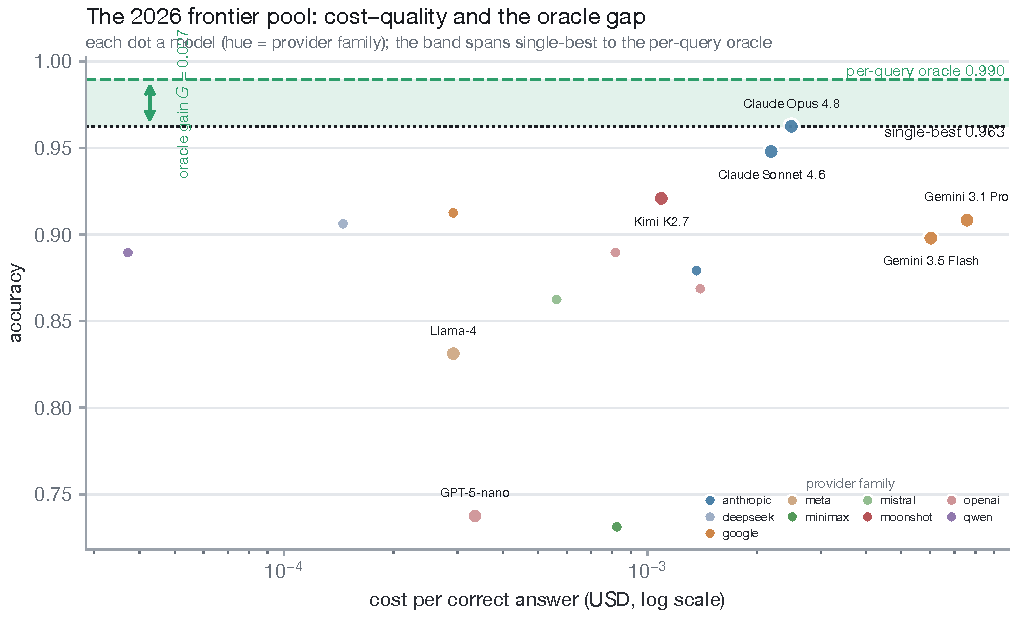
\includegraphics[width=\textwidth]{figures/fig_cost_quality.pdf}
\caption{\label{fig:cq}Pillar A cost--quality frontier (re-graded): the per-query oracle (green) sits just above single-best
(black); cheap models populate the frontier.}
\end{minipage}\hfill
\begin{minipage}{0.49\textwidth}\centering
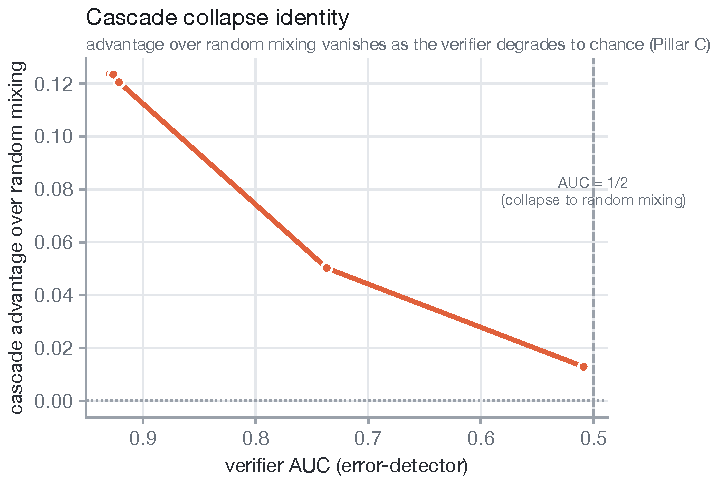
\includegraphics[width=\textwidth]{figures/fig_cascade_collapse.pdf}
\caption{\label{fig:casc}Pillar C: the cascade's advantage over random-mixing-at-matched-budget collapses to zero as the
verifier's AUC falls to $\tfrac12$, confirming Eq.~\eqref{eq:collapse}.}
\end{minipage}
\end{figure}
\begin{figure}[tbp]
\begin{minipage}{0.49\textwidth}\centering
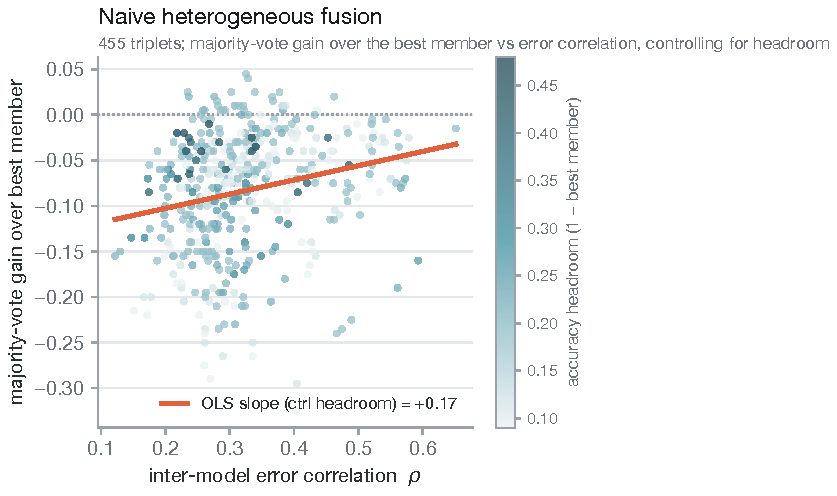
\includegraphics[width=\textwidth]{figures/fig_rho_gain.pdf}
\caption{\label{fig:rho}Pillar B, 455 triplets: unweighted majority-vote gain over the best member vs.\ $\rho$; the gain is negative
for most triplets; its slope on $\rho$ has the opposite sign to the diversification prediction and is not significant under
model-clustering.}
\end{minipage}\hfill
\begin{minipage}{0.49\textwidth}\centering
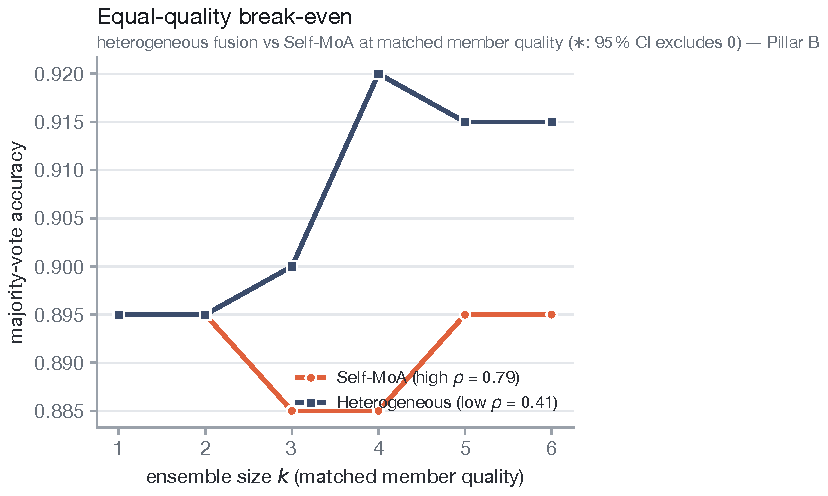
\includegraphics[width=\textwidth]{figures/fig_equal_quality.pdf}
\caption{\label{fig:eqq}Equal-quality break-even ($S{=}9$, matched 6-model band): low-$\rho$ heterogeneous fusion ($\rho{=}\nEqRhoHet$)
vs.\ high-$\rho$ Self-MoA ($\rho{=}\nEqRhoSelf$), both on distinct draws so Self-MoA scales without recycling samples. Under the primary
distinct-draw aggregation the heterogeneous ensemble is ahead of Self-MoA from the information-fair $k{=}3$ onward, by at most
$\nEqBestDiff$; the query-bootstrap 95\% CI excludes zero only at $k{=}\nEqSigK$ ($\ast$).}
\end{minipage}
\end{figure}
\begin{figure}[tbp]\centering
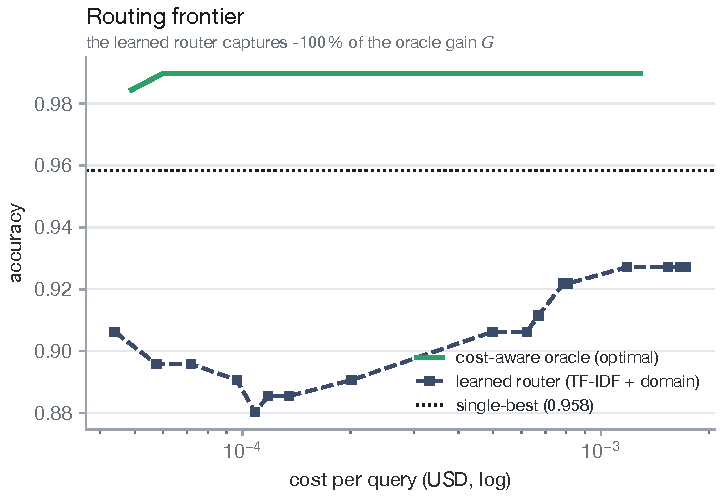
\includegraphics[width=0.55\textwidth]{figures/fig_router.pdf}
\caption{\label{fig:router}Pillar A, realizable routing: a held-out learned router (TF-IDF$+$domain) vs.\ the cost-aware oracle
(optimal) frontier and single-best, on the multi-domain mix. The learned router falls below single-best (captures $\nRtFracPct\%$ of
$G$; 95\% CI excludes zero) and far below the optimal frontier; realizable routing gain is zero or negative.}
\end{figure}

\section{Discussion}\label{sec:disc}
\textbf{One allocation problem on two timescales.} The results are not separate vignettes but one allocation problem viewed
at two timescales. Within a release epoch, prices and the pool are fixed and the buyer solves the static allocation of
App.~\ref{sec:A}--\ref{sec:C}: a budget-priced assignment with value $V(B)$ and shadow price $\lambda_B$ (Prop.~\ref{prop:duality}),
capped by the realizability ceiling (Prop.~\ref{prop:cert}). Across epochs, frontier releases arrive and the buyer holds an
option on the next pool; the option value of breadth (App.~\ref{app:churn}) is the continuation value attached to that stage
problem. This is a decomposition that organizes the results rather than a solved Bellman system (the churn primitives
$(\nu,\Gamma,v)$ are not derived from the stage problem), and its continuation algebra is standard real-options machinery. With that:
routing value is a first-moment selection effect that scales with dispersion rather than capability (App.~\ref{sec:A}); fusion value is a
second-moment effect bounded by systematic error and, empirically, a point or two even under accuracy-matched combination
(App.~\ref{sec:B});
cascade value is a decision-theoretic effect whose integral over escalation budgets is exactly $a_L(1-a_L)(\mathrm{AUC}-\tfrac12)$, the
verifier's AUC lift over chance (App.~\ref{sec:C}). Because all three
shrink as the frontier converges and errors correlate (Cor.~\ref{cor:converge}), the value of a routing layer tracks market churn and
heterogeneity, not the absolute capability of the best model (App.~\ref{app:churn}). The empirical signature on the 2026 frontier is a ceiling at $1$ with the best model already on it: where the frontier is
strong (MATH-500, MATH-Hard), oracle gains are a point or two; where it is weaker (AIME, GPQA), the gains are larger but they
are disagreements, and exploiting them needs a per-query signal that none of our routers finds. \emph{Naive} fusion is worse
than useless: unequal members outvote the strongest one (\S\ref{sec:results}).

\section{Limitations}\label{sec:limits}
\textbf{Where a tail might exist.} Our benchmarks are ones on which the 2026 frontier is strong, and on all of them the audited
$\beta$ is zero or close to it. A genuine co-failure tail may well exist on harder workloads---research-level mathematics,
long-horizon agentic tasks, or code at a difficulty where the frontier fails---and there the underpricing of
Prop.~\ref{prop:poolbias} would matter; the certificate and the audit protocol apply unchanged, but we have not measured such a
tail.
\textbf{Grading.} Programmatic grading covers verifiable tasks only. Our math normalization follows the MATH benchmark's reference
evaluation and a symbolic fallback, but it can still miss unusual equivalent forms (an implicit product such as $2\sqrt3$ written
without a multiplication sign does not parse symbolically); every all-wrong question is audited, and every all-wrong event the corrected grader resolved was resolved by
answers equal to the reference (\texttt{audit/grader\_resolved.json}), but a grader false positive elsewhere could hide an all-wrong
question; every grade can be re-checked from the released responses. The only genuine co-failures arise under direct-answer
prompting. Free-response GPQA is graded by an LLM panel, not by humans. The
adjudication and the GPQA screen used AI raters; human raters would be stronger.
\textbf{Economics and pillars.} The static-price assumptions of App.~\ref{sec:A}--\ref{sec:C} are in tension with the churn of
App.~\ref{app:churn}; those claims are restricted to within-release-epoch validity. The sensitivity $\lambda$ is derived as a
decision-rule Jacobian (Prop.~\ref{prop:lambda}), but its empirical fit across $\rho$ levels and out-of-sample prediction of
$k^\ast$ remain open, and the matched-quality test rests on one provider-matched band. Inference on the unconditional
$\rho$-slope is inconclusive under model-clustering; $G$ and the block-$\rho$ gap are reported without seed replication. The churn
study (App.~\ref{app:churn}) is stylized and observational. The routers are trained on the 15-model pool only; the
market-scale routing statement rests on the certificate. The cascade is measured against a naive confidence cascade, not the
optimal cascade-routing policy of \citet{dekoninck2024cascaderouting}, and its verifier scores only the cheap model, whereas the
optimal deferral rule conditions on both \citep{jitkrittum2023cascade}.

\section{Conclusion}
The field decides whether to orchestrate by reading one number, pairwise error correlation, and that number is blind to the
joint failures that set the ceiling. The right object is $\beta$, the co-failure rate, and a \$0 certificate on it says
before any router is built how much orchestration can gain. Measured on $\nMathM$ models and audited question by question, the
verdict is clear: no mathematics or science question in our benchmarks defeats every model, the best single model already sits
at the ceiling where the frontier is strong, and no router we train captures the headroom that remains. Combining models rarely
beats the single best model, and the reason is not that models fail together. The one co-failure tail we measured was our own
evaluation's making, and it fooled a pairwise model the way the theory predicts; reading the all-wrong questions caught it.
The rule for practice: certify $\beta$ before you build a router (one line on any 0/1 grade matrix with our released
\texttt{beta\_certificate.py}), and audit every all-wrong question before you trust the certificate. Whether a genuine co-failure tail appears on harder workloads, such as research-level mathematics or long-horizon
agents, is the open question.

\bibliographystyle{plainnat}
\bibliography{references}

\appendix
\section{Economic scaffolding: routing, diversification, and cascades}\label{app:econ}
This appendix gives the economic scaffolding deferred from the main text (\S\ref{sec:setup-formal}); its tools are standard, and the empirical claims do not rest on it.

\subsection{Routing as priced assignment}\label{sec:A}
\emph{The envelope and dispersion-scaling material below is background, claimed by no one}: the oracle envelope and the
value-of-information gap are textbook \citep{howard1966}, and routing optimality is proven by
\citet{dekoninck2024cascaderouting}. Proposition~\ref{prop:duality} makes ``orchestration
is allocation'' literal: under a dollar budget, routing is a priced assignment with an explicit shadow price.

\begin{lemma}[Envelope and dominance condition; background]\label{lem:env}
For every routing policy $\pi$, $V(\pi)\le V^o:=\E_t\max_i q_i(t)$, attained by the oracle $\pi^o(t)=\arg\max_i q_i(t)$.
Let the oracle gain be $G:=V^o-\max_i\bar q_i\ge 0$. Then $G>0$ iff no model is uniformly best across types
$D$-almost everywhere; equivalently, the quality matrix $Q=[q_i(t)]$ is not row-dominated under $D$.
\end{lemma}

\begin{proposition}[Budget-constrained routing: shadow price and bang-per-buck rule]\label{prop:duality}
Fix a dollar budget $B$ and let $V(B)=\max_{\pi}\{V(\pi):K(\pi)\le B\}$ over routing policies. This is a linear program
whose dual collapses to a \emph{single scalar} price $\lambda_B\ge0$ on the budget,
\[ V(B)=\min_{\lambda\ge0}\Big\{\lambda B+\E_t\max_i\big[q_i(t)-\lambda c_i\big]\Big\}, \]
because the per-type simplex constraints are absorbed pointwise. Every optimal policy routes type $t$ to
$\arg\max_i[q_i(t)-\lambda_B c_i]$, a per-type \emph{bang-per-buck} rule, mixing only where the budget binds. The value
$V(B)$ is nondecreasing, concave, and piecewise linear, with $V'(B)=\lambda_B$ wherever differentiable; once $B$ exceeds
the oracle's cost, $\lambda_B=0$ and the rule is the unconstrained per-query oracle.
\end{proposition}
\noindent This specializes standard linear-programming duality \citep{bertsimas1997lp} to inference routing. The step
is small but earns the allocation framing: orchestration under a budget is a priced assignment, and $\lambda_B$, the
\emph{shadow price of the inference dollar}, is the price a budget-aware buyer trades quality against (the same dollars-per-correct
currency the cost-aware rules of \S\ref{sec:B}--\ref{sec:C} optimize). With several resources (e.g.\ dollars and latency) $\lambda_B$ becomes a vector and the score is
$q_i(t)-\lambda_B\!\cdot c_i$. We verified the dual price, the bang-per-buck characterization, and concavity numerically.

\noindent\textbf{Dispersion scaling (heuristic).} If, purely as an illustration, the cell qualities $q_i(t)$ were i.i.d.\
$\mathcal N(\mu,s^2)$ across the $m\times|T|$ cells with $|T|$ large relative to $\ln m$, then $V^o\approx\mu+s\sqrt{2\ln m}$
while the best row mean concentrates at $\mu$, giving $G\sim s\sqrt{2\ln m}$: linear in cross-model within-type dispersion
$s$, only logarithmic in pool size $m$. We flag this as heuristic: real errors are block-correlated (\S\ref{sec:results}),
which lowers the rate, but the qualitative message (value from \emph{how} models differ, not how many) is what the
empirics test. A learned router with expected routing regret $R$ attains $V^o-R$ and beats single-best iff $R<G$. As $G$
is monotone in partition fineness, we report a partition-free per-query oracle as the true upper bound.

\subsection{The cost-aware diversification limit}\label{sec:B}
Let model errors satisfy $\Var(e_i)=\sigma^2$ and $\Corr(e_i,e_j)=\rho$, with systematic variance $\tau^2=\rho\sigma^2$
and idiosyncratic variance $(1-\rho)\sigma^2$.

\begin{proposition}[Variance floor (classical)]\label{prop:floor}
Equal-weight fusion of $k$ equicorrelated models has mean-squared error $V(k)=\sigma^2(\rho+\tfrac{1-\rho}{k})\to\rho\sigma^2$.
Under a symmetric single-factor probit with per-model error rate $\alpha<\tfrac12$, unweighted majority vote has infinite-ensemble
error floor $\Phi(-\Phi^{-1}(1-\alpha)/\sqrt\rho)$, with limits $0$ ($\rho\to0$) and $\alpha$ ($\rho\to1$).
\end{proposition}
\noindent The continuous floor is the equicorrelated portfolio-variance limit \citep{markowitz1952,statman1987} and the
bias--variance--covariance/diversity decomposition \citep{ueda1996,krogh1995ensemble,wood2023diversity}; the copula floor is
\citet{turkmen2026ensembleselection}; all three are classical.

\begin{proposition}[Cost-aware break-even]\label{prop:keven}
Let $\lambda$ be the local sensitivity of expected correctness to fused-estimate variance for the operative decision rule,
$\lambda := -\,\partial(\text{expected correct})/\partial V$, evaluated near the operating point (a derived Jacobian for a
threshold rule, not a risk-aversion parameter; under strict risk neutrality $\lambda$ is the local curvature through which
second moments enter the first-moment objective). With per-model cost $c$ and $\lambda>0$, growing the ensemble from $k$ to
$k{+}1$ members pays for itself iff $k\le k^\ast$, where
\begin{equation}
k^\ast(\rho,c)=\tfrac12\Big(-1+\sqrt{1+4\lambda\sigma^2(1-\rho)/c}\Big),\qquad
k^\ast\sim\sqrt{\lambda\sigma^2(1-\rho)/c}.\label{eq:keven}
\end{equation}
Hence, holding $\lambda$ fixed, $\partial k^\ast/\partial\rho<0$, $\partial k^\ast/\partial c<0$, and $\rho\to1\Rightarrow k^\ast\to0$. The optimal
ensemble cardinality is $\lfloor k^\ast\rfloor{+}1$.
\end{proposition}

\begin{proposition}[Calibration of $\lambda$ and a sign condition]\label{prop:lambda}
Under the symmetric single-factor probit of Prop.~\ref{prop:floor} (latent $S_i=\mu_\alpha+\sqrt\rho\,U+\sqrt{1-\rho}\,\xi_i$,
$\mu_\alpha=\Phi^{-1}(1-\alpha)$, correct iff $S_i>0$; $\sigma^2=1$), equal-weight fusion has fused score $Z_k\sim\mathcal N(\mu_\alpha,V(k))$, and the
risk-neutral mean-score vote (correct iff $Z_k>0$; it coincides with majority vote as $k\to\infty$) has expected correctness
$P(V)=\Phi(\mu_\alpha/\sqrt V)$ in the single sufficient statistic $V=V(k)$. The sensitivity $\lambda$ in \eqref{eq:keven} is then
not a free parameter but the explicit Jacobian
\[ \lambda(V)=-\frac{\partial P}{\partial V}=\frac{\mu_\alpha}{2V^{3/2}}\,\varphi\!\Big(\frac{\mu_\alpha}{\sqrt V}\Big),\qquad \mu_\alpha=\Phi^{-1}(1-\alpha), \]
evaluated at the operating point $V=V(k)$. Its sign is $\operatorname{sgn}\lambda=\operatorname{sgn}(\tfrac12-\alpha)$: when
each member beats chance ($\alpha<\tfrac12$), $\lambda>0$ and $P$ strictly decreases in $V$, so reducing $V$ by adding members
strictly raises expected correctness and $k^\ast$ is well defined; at $\alpha>\tfrac12$, $\lambda<0$ and the diversification
framing fails (adding members drives the vote \emph{more} wrong, and \eqref{eq:keven} returns no positive $k^\ast$).
\end{proposition}
\noindent This pins down the economic bridge the cost-aware rule rests on and delimits where it is valid. $\lambda$ is an
operating-point Jacobian (it depends on $V$, hence weakly on $k$); we evaluate it at the marginal index, where the
local-linearization error is second order in the step, $O(\Delta V(k)^2)=O\big((1-\rho)^2/k^4\big)$. A finite-sample estimator plugs the tetrachoric $\hat\rho$ and per-model
$\hat\alpha$ into $\lambda(V(k))$; the Pearson coefficient of $0/1$ indicators biases $\rho$ downward and so distorts $\lambda$. We
verified $\lambda=-\partial P/\partial V$ and the sign condition numerically.

\paragraph{Query-conditional $\rho$ and block covariance.} Classical $\rho$ is a global constant; making $\rho(t)$
type-conditional makes $k^\ast$ vary within a single workload and resolves the diversity-unreliability result
\citep{kuncheva2003} by conditioning. Because errors are block-structured and rise with accuracy \citep{kim2025correlated},
the headline object is the block covariance $\Sigma$: equal weights are no longer optimal (the minimum-variance weights are
$w\propto\Sigma^{-1}\mathbf 1$), and the floor is the undiversifiable common-factor component of $\Sigma$. The equicorrelation
form is the special case. We caution that the portfolio analogy is a first-moment-plus-local-curvature analogy, not a claim of
risk aversion.

\begin{figure}[tbp]\centering
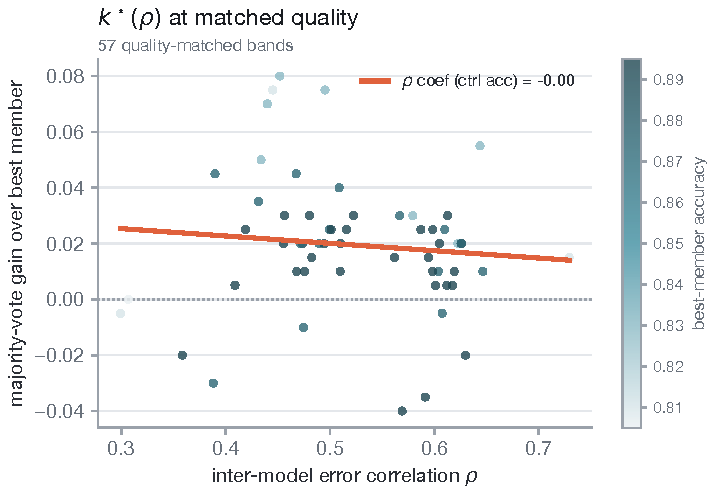
\includegraphics[width=0.55\textwidth]{figures/fig_kstar.pdf}
\caption{\label{fig:kstar}Pillar B, $k^\ast(\rho)$ at matched quality: across \nKsBands{} sub-bands of the matched 6-model pool (MMLU-Pro),
majority-vote gain over the best member vs.\ inter-model $\rho$, controlling for member accuracy. The slope is
indistinguishable from zero ($\nKsSlopeSix$, CI $[\nKsSlopeSixLo,\nKsSlopeSixHi]$), as it is on the 9-model band ($\nKsSlopeNine$).}
\end{figure}

\subsection{Cascade calibration economics}\label{sec:C}
A cheap model $L$ (price $c_L$, accuracy $a_L$) answers first with confidence $s$; the query escalates to a strong model $H$
when $s<\tau$. (We write $\gamma$ for the escalation fraction to keep $\beta$ for the co-failure rate.) Let $\gamma=\Pr[s<\tau]$ be
the escalation budget, $w(\gamma)=\Pr[Y_L=0\mid\text{escalated }\gamma\text{-tail}]$ the tail error rate, and $a_H(\tau)$ the strong
model's accuracy on the deferred tail. Then $C(\gamma)=c_L+\gamma c_H$ and $Q(\gamma)=a_L+\gamma[a_H(\tau)-1+w(\gamma)]$.

\begin{proposition}[Collapse, ceiling, dominance]\label{prop:cascade}
Against random mixing (escalate a random $\gamma$-fraction; tail error $1-a_L$, tail accuracy $a_H$) at equal budget,
\begin{equation}
Q(\gamma)-Q_{\mathrm{mix}}(\gamma)=\gamma\big[w(\gamma)-(1-a_L)\big]+\gamma\big[a_H(\tau)-a_H\big].\label{eq:collapse}
\end{equation}
If $a_H(\tau)=a_H$ (no tail adverse selection) and $s$ has no ties, the integrated advantage is exactly
\[ \int_0^1\big[Q(\gamma)-Q_{\mathrm{mix}}(\gamma)\big]\,d\gamma=\int_0^1\gamma\big[w(\gamma)-(1-a_L)\big]\,d\gamma=a_L(1-a_L)\big(\mathrm{AUC}-\tfrac12\big), \]
where AUC is the probability that the verifier scores a random error of $L$ below a random success. It is therefore
$\ge0$ iff $\mathrm{AUC}\ge\tfrac12$, with equality iff $\mathrm{AUC}=\tfrac12$ (for $0<a_L<1$), and the cascade then does no
better than random mixing on average. Pointwise nonnegativity is guaranteed when $w$ is non-increasing (a threshold-rational
verifier), since $w(1)=1-a_L$. Under perfect calibration the escalation ratio is
$\gamma_{\mathrm{cas}}/\gamma_{\mathrm{mix}}=1-a_L/a_H$: relative to random mixing, a calibrated cascade
needs only a fraction $1-a_L/a_H$ as many strong-model calls at a fixed quality floor, independent of price. Within a
one-parameter family of verifiers ordered by AUC, $\gamma_{\mathrm{cas}}(q)$ is decreasing in AUC, so a critical
$\mathrm{AUC}^\ast$ exists below which (given $c_L/c_H<q/a_H$) no threshold meets floor $q\in(a_L,a_H]$ at lower
dollars-per-correct than the strong model alone.
\end{proposition}

\begin{corollary}[Calibration-and-edge: necessary condition]\label{cor:edge}
Cascade dominance over $H$-only requires both $\mathrm{AUC}(s)>\mathrm{AUC}^\ast$ and a positive conditional edge
$a_H(\tau)>a_L(\tau)$ on the deferred tail. If $H$ is adversely weak where $L$ defers, calibration alone is insufficient
(consistent with \citealp{jitkrittum2023cascade}).
\end{corollary}

% Optionality under churn (formerly Pillar D) relocated to App.~\ref{app:churn} as a secondary, observational result.

\section{Proofs}\label{app:proofs}
\begin{proof}[Proof of Lemma~\ref{lem:env}]
For any $\pi$ and $t$, $\sum_i\pi(i\mid t)q_i(t)\le\max_i q_i(t)$; take $\E_t$ to get $V(\pi)\le V^o$, attained by $\pi^o$. Write
$G=\E_t[\max_i q_i(t)-q_{i^\ast}(t)]$ with $i^\ast=\arg\max_i\bar q_i$; the integrand is nonnegative. If model $j$ is uniformly best
$D$-a.e.\ then $\bar q_j=V^o$, so $G=0$; conversely, if no model is uniformly best, the set where $i^\ast$ is suboptimal has positive
measure and the integrand is strictly positive there, so $G>0$. The dispersion-scaling remark uses the extreme-value asymptotic
$\E[\max$ of $m$ i.i.d.\ $\mathcal N(0,1)]\sim\sqrt{2\ln m}$ and concentration of the best row mean at $\mu$ when $|T|\gg\ln m$; it is
heuristic under correlation.
\end{proof}
\begin{proof}[Proof of Prop.~\ref{prop:floor}]
With $e_i=b+\varepsilon_i$, $\Var(b)=\rho\sigma^2$, $\Var(\varepsilon_i)=(1-\rho)\sigma^2$ uncorrelated, the equal-weight average has
$\Var(\bar e)=\rho\sigma^2+(1-\rho)\sigma^2/k\to\rho\sigma^2$. For binary correctness under $S_i=\mu_\alpha+\sqrt\rho\,U+\sqrt{1-\rho}\,\xi_i$ with
$\mu_\alpha=\Phi^{-1}(1-\alpha)$, conditioning on $U$ gives correctness probability $\Phi((\mu_\alpha+\sqrt\rho U)/\sqrt{1-\rho})$; by the law of large
numbers the majority is correct iff that probability exceeds $\tfrac12$, i.e.\ iff $U>-\mu_\alpha/\sqrt\rho$, so the floor is
$\Phi(-\mu_\alpha/\sqrt\rho)$. As $\rho\to1$ it tends to $\Phi(-\mu_\alpha)=\alpha$; as $\rho\to0$ it tends to $0$ because $\mu_\alpha>0$ when $\alpha<\tfrac12$.
\end{proof}
\begin{proof}[Proof of Prop.~\ref{prop:keven}]
Growing the ensemble from $k$ to $k{+}1$ members reduces variance by $\Delta V(k)=V(k)-V(k{+}1)=\sigma^2(1-\rho)/[k(k+1)]$. Converting to expected correctness
through the local sensitivity $\lambda>0$, the step is worthwhile iff $\lambda\,\Delta V(k)\ge c$, i.e.\ $k(k+1)\le R$ with
$R=\lambda\sigma^2(1-\rho)/c$. Since $k(k+1)$ is increasing, this holds iff $k\le k^\ast$, the positive root of $k(k+1)=R$, which is
\eqref{eq:keven}. Members are therefore added for $k=1,\dots,\lfloor k^\ast\rfloor$, and the optimal cardinality is $\lfloor k^\ast\rfloor+1$.
With $\lambda$ held fixed the comparative statics follow by inspection, and $R\to0$ as $\rho\to1$.
\end{proof}
\begin{proof}[Proof of Prop.~\ref{prop:cascade} and Cor.~\ref{cor:edge}]
Escalated mass $\gamma$ pays $c_H$ on top of $c_L$, giving $C(\gamma)=c_L+\gamma c_H$. On the escalated tail (mass $\gamma$, of which $L$
answered a fraction $1-w(\gamma)$ correctly) $L$'s answers are replaced by $H$ scoring $a_H(\tau)$, giving
$Q(\gamma)=a_L-\gamma(1-w(\gamma))+\gamma a_H(\tau)=a_L+\gamma[a_H(\tau)-1+w(\gamma)]$. Random mixing
escalates a random $\gamma$-fraction with tail error $1-a_L$ and tail accuracy $a_H$, giving $Q_{\mathrm{mix}}=a_L+\gamma(a_H-a_L)$;
subtracting yields \eqref{eq:collapse}. With $a_H(\tau)=a_H$ the advantage is $\gamma[w(\gamma)-(1-a_L)]=E(\gamma)-(1-a_L)\gamma$, where
$E(\gamma)$ is $L$'s error mass in the escalated tail. Writing $E(\gamma)=(1-a_L)\,T(\gamma)$ with $T$ the fraction of $L$'s errors caught
(the cumulative-gains curve of $s$), the classical identity $\int_0^1[T(\gamma)-\gamma]\,d\gamma=a_L(\mathrm{AUC}-\tfrac12)$ for a
cumulative-gains curve with positive rate $1-a_L$ gives $\int_0^1\gamma[w(\gamma)-(1-a_L)]\,d\gamma=a_L(1-a_L)(\mathrm{AUC}-\tfrac12)$.
Pointwise, $w$ non-increasing with $w(1)=1-a_L$ gives $w(\gamma)\ge1-a_L$ for all $\gamma$. Under perfect calibration the escalated tail
is exactly $L$'s errors until exhausted, so $Q(\gamma)=a_L+\gamma a_H$ for $\gamma\le 1-a_L$, whence $\gamma_{\mathrm{cas}}(q)=(q-a_L)/a_H$;
since $\gamma_{\mathrm{mix}}(q)=(q-a_L)/(a_H-a_L)$, the ratio is $\gamma_{\mathrm{cas}}/\gamma_{\mathrm{mix}}=1-a_L/a_H$. Beating
$H$-only ($c_H/a_H$ per correct) at floor $q$ requires $c_L+\gamma_{\mathrm{cas}}(q)c_H\le(q/a_H)c_H$, feasible only if $c_L/c_H<q/a_H$;
within a one-parameter AUC-ordered family $\gamma_{\mathrm{cas}}$ decreases in AUC, so $\mathrm{AUC}^\ast$ exists. If $a_H(\tau)\le a_L(\tau)$
on the deferred tail, escalation cannot raise quality there, so no $\tau$ achieves $q$: dominance requires both AUC above threshold and a
positive tail edge. We prove necessity; sufficiency additionally needs reachability of $q$ and the cost ordering.
\end{proof}
\begin{proof}[Proof of Prop.~\ref{prop:option}]
The captured value per arrival is $v\,\E[\max(\Gamma,0)]=v\,\mathrm{Eg}$ by the Gaussian truncation identity. A captured lead is held for an
$\mathrm{Exp}(\nu)$ time and discounted at $r$ (factor $1/(r+\nu)$); the Poisson arrival stream contributes a present-value
multiplier $\nu/r$, giving $V_R=v\,\mathrm{Eg}\cdot\nu/(r+\nu)\cdot(1/r)$. Then $\partial\mathrm{Eg}/\partial\eta=\varphi(\mu/\eta)>0$
and $\partial[\nu/(r+\nu)]/\partial\nu>0$; adding a separable $m(\text{level})$ leaves both partials unchanged.
\end{proof}
\begin{proof}[Proof of Prop.~\ref{prop:duality}]
$(P_B)$ is linear in $\{\pi(i\mid t)\}$. Dualize only the budget row with multiplier $\lambda\ge0$, keeping the per-type
simplices as the domain; the Lagrangian separates across $t$ into inner problems
$\max_{\pi(\cdot\mid t)\in\Delta}\sum_i\pi(i\mid t)(q_i(t)-\lambda c_i)=\max_i(q_i(t)-\lambda c_i)=:g_t(\lambda)$. Weak duality
gives $V(B)\le\lambda B+\E_t g_t(\lambda)$ for every $\lambda\ge0$; LP strong duality (Slater holds for $B>\underline B$) gives
equality at some $\lambda_B$. Complementary slackness places every optimal $\pi^\star(\cdot\mid t)$ on
$\arg\max_i(q_i(t)-\lambda_B c_i)$, mixing only to exhaust the budget. As a minimum of affine functions of $B$, $V$ is concave;
it is nondecreasing (enlarging $B$ relaxes a constraint) and piecewise linear (parametric LP). By the envelope theorem
$V'(B)=\lambda_B$ where differentiable, with subdifferential $[\lambda_B^-,\lambda_B^+]$ at the finitely many kinks; once
$B\ge K(\pi^o)$ the budget is slack, $\lambda_B=0$, and the rule is the per-query oracle.
\end{proof}
\begin{proof}[Proof of Prop.~\ref{prop:lambda}]
Under the single-factor probit, $Z_k=\tfrac1k\sum_i S_i=\mu_\alpha+\sqrt\rho\,U+\tfrac{\sqrt{1-\rho}}{k}\sum_i\xi_i\sim\mathcal N(\mu_\alpha,V(k))$,
$V(k)=\rho+(1-\rho)/k$ ($\sigma^2{=}1$). The mean-score vote is correct iff $Z_k>0$, so $P(V)=\Pr[Z_k>0]=\Phi(\mu_\alpha/\sqrt V)$.
Then $\partial P/\partial V=\varphi(\mu_\alpha/\sqrt V)\cdot \mu_\alpha\cdot(-\tfrac12)V^{-3/2}$, so $\lambda:=-\partial P/\partial V=(\mu_\alpha/2V^{3/2})\varphi(\mu_\alpha/\sqrt V)$.
As $\varphi>0,V>0$, $\operatorname{sgn}\lambda=\operatorname{sgn}\mu_\alpha=\operatorname{sgn}(\Phi^{-1}(1-\alpha))=\operatorname{sgn}(\tfrac12-\alpha)$.
Substituting $\lambda$ into $\lambda\,\Delta V(k)\ge c$ with $\Delta V(k)=(1-\rho)/[k(k+1)]$ reproduces \eqref{eq:keven}.
\end{proof}
\begin{proof}[Proof of Prop.~\ref{prop:cert}]
(i) On the all-wrong event every member answer differs from the label; a selection policy outputs one member answer, hence is
wrong there, so $\mathrm{Acc}(\pi)\le\Pr[\text{not all wrong}]=1-\beta$, attained by the per-query oracle. (ii)
$V^o=\E_t\mathbf 1\{\exists i:Y_i{=}1\}=1-\beta$ and $a_{\mathrm{sb}}=\Pr[Y_{i^\star}{=}1]$, so
$G=V^o-a_{\mathrm{sb}}=\Pr[Y_{i^\star}{=}0]-\beta=\Pr[\text{single-best wrong}]-\beta$, the non-unanimous single-best-wrong mass.
(iii) $K=\sum_j\mathbf 1\{\text{all wrong on }t_j\}\sim\mathrm{Binomial}(n,\beta)$ since the $t_j$ are i.i.d.\ and ``all wrong''
is a fixed event; the Clopper--Pearson lower limit obeys $\Pr[\beta\ge\beta_{\mathrm{lo}}]\ge1-\delta$, so with probability
$\ge1-\delta$, $(1-\beta)\le(1-\beta_{\mathrm{lo}})$ and every selection policy obeys
$\mathrm{Acc}-a_{\mathrm{sb}}\le(1-\beta)-a_{\mathrm{sb}}\le(1-\beta_{\mathrm{lo}})-a_{\mathrm{sb}}$. If $a_{\mathrm{sb}}$ is itself
estimated, let $a_{\mathrm{sb}}^{\mathrm{lo}}$ be a lower confidence bound at level $1-\delta'$ (e.g.\ Clopper--Pearson for any fixed
model, since $a_{\mathrm{sb}}$ is at least that model's accuracy); on the event $a_{\mathrm{sb}}\ge a_{\mathrm{sb}}^{\mathrm{lo}}$,
$(1-\beta_{\mathrm{lo}})-a_{\mathrm{sb}}\le(1-\beta_{\mathrm{lo}})-a_{\mathrm{sb}}^{\mathrm{lo}}$, and a union bound gives total error
$\le\delta+\delta'$. (An \emph{upper} bound on $a_{\mathrm{sb}}$ would shrink the certified gain and is not valid.)
\end{proof}
\begin{proof}[Proof of Prop.~\ref{prop:poolbias}]
$\beta(m)=\omega+(1-\omega)\alpha_0^{\,m}$ is strictly decreasing to $\omega$ since $0<\alpha_0<1$. Calibrate the single-factor Gaussian
copula to reproduce the marginal $\alpha$ and the pairwise co-error $\omega+(1-\omega)\alpha_0^2\in(\alpha^2,\alpha)$, which fixes a unique
latent correlation $r:=\rho_{\mathrm{tet}}\in(0,1)$; then $\beta_{\mathrm{sf}}(2)=\omega+(1-\omega)\alpha_0^2=\beta(2)$, so the ratio is $1$ at $m=2$. For $m\ge2$, conditioning
on the common factor $Z$, $\beta_{\mathrm{sf}}(m)=\E[p(Z)^m]$ with $p(z)=\Phi\big((z_\alpha-\sqrt{r}\,z)/\sqrt{1-r}\big)$ and
$z_\alpha=\Phi^{-1}(\alpha)$. For each fixed $z$, $p(z)\in(0,1)$ since $r<1$, so $p(z)^m\to0$ pointwise; dominated convergence gives
$\beta_{\mathrm{sf}}(m)\to0$ (this is the zero lower-tail-dependence of the Gaussian copula, \citealp{embrechts2002correlation}). Since
$\beta(m)\to\omega>0$ and $\beta_{\mathrm{sf}}(m)\to0$, the ratio $R(m):=\beta(m)/\beta_{\mathrm{sf}}(m)\to\infty$.

For eventual monotonicity, compare the two successive ratios. First, $1-\beta(m{+}1)/\beta(m)=(1-\omega)(1-\alpha_0)\alpha_0^m/\beta(m)\le C\alpha_0^m$
with $C=(1-\omega)(1-\alpha_0)/\omega$: $\beta$ converges geometrically. Second, $\beta_{\mathrm{sf}}$ decays only polynomially. The
variable $p(Z)$ has the Vasicek law, whose density near $1$ is $(1-x)^{\chi-1}e^{O(\sqrt{\log(1/(1-x))})}$ with $\chi=(1-r)/r>0$, so
Laplace's method gives $\beta_{\mathrm{sf}}(m)=m^{-\chi+o(1)}$. (In particular $\beta_{\mathrm{sf}}(m{+}1)/\beta_{\mathrm{sf}}(m)\to1$ as well;
what matters is the rate.) Also $s_m:=\beta_{\mathrm{sf}}(m{+}1)/\beta_{\mathrm{sf}}(m)$ is non-decreasing in $m$, because the moments of
$p(Z)\in[0,1]$ are log-convex by Cauchy--Schwarz. Suppose $R(m{+}1)\le R(m)$ for infinitely many $m$, i.e.\
$s_m\ge\beta(m{+}1)/\beta(m)\ge1-C\alpha_0^m$. Put $N_m=\lceil\alpha_0^{-m}\rceil$. Monotonicity of $s$ gives
$\beta_{\mathrm{sf}}(m{+}N_m)\ge\beta_{\mathrm{sf}}(m)(1-C\alpha_0^m)^{N_m}\ge\beta_{\mathrm{sf}}(m)\,e^{-2C}$ for large such $m$. But the left side is
$\exp\{-(\chi+o(1))\,m\log(1/\alpha_0)\}$ and the right side is $\exp\{-(\chi+o(1))\log m\}$, a contradiction for large $m$. Hence $R$
is eventually strictly increasing (numerically, strictly from $m{=}2$ in all settings we tested).
\end{proof}
\begin{proof}[Proof of Prop.~\ref{prop:nonid}]
Take exchangeable error triples on $\{0,1\}^3$ and let $q_j$ be the probability of exactly $j$ errors ($\sum_j q_j=1$). Every
pair has the same $2{\times}2$ table, determined by the marginal error rate $p_1=\tfrac13\sum_j j\,q_j$ and the pairwise
co-error $p_2=\Pr[X_i{=}X_j{=}1]=\tfrac13(q_2+3q_3)$; the triple-failure cell $\beta=q_3$ is left free in the resulting
one-parameter Fr\'echet class. Concretely, fix $p_1=\tfrac12,\ p_2=\tfrac14$: both $(q_0,q_1,q_2,q_3)=(\tfrac14,0,\tfrac34,0)$
and $(0,\tfrac34,0,\tfrac14)$ reproduce \emph{every} one- and two-dimensional marginal---hence every pairwise Pearson and
tetrachoric correlation, which are functions of that common bivariate table---yet have $\beta=0$ and $\beta=\tfrac14$. So
$\beta$ is not a function of the pairwise law. Padding with independent coordinates extends the example to any $m\ge3$, and the
common-shock mixture ($\beta_\infty=\omega>0$) versus a matched-$\bar\rho$ Gaussian copula ($\beta_\infty=0$ by zero lower
tail dependence) realize the two extremes as $m\to\infty$, both consistent with the same pairwise $\bar\rho$.
\end{proof}

\section{Reproducibility}\label{app:repro}
\textbf{Code, data, and a one-command check.} Everything needed to regenerate every number and figure in this paper is
public: code at \url{https://github.com/josefchen/co-failure-ceiling}, data at
\url{https://huggingface.co/datasets/josefchen/co-failure-67-models} (fetched at a pinned revision by
\texttt{scripts/fetch\_data.py}), and an interactive companion at
\url{https://huggingface.co/spaces/josefchen/orchestration-is-allocation}. The data are the per-cell outcome matrices (every
model's graded correctness, token counts, and metered cost on every query), the exact question text, reference answer, and
token budget of every item (\texttt{items\_snapshot.json}), the raw model response behind every graded cell, the judge votes,
the model registry with dated snapshots and prices, and a per-cell log of every re-run. We also release the benchmark
errata the audit produced: wrong and ambiguous reference answers in MATH-Hard, MMLU-Pro, MMLU, GSM8K and ARC, and the
MATH-500 and MATH-Hard questions a naive grader marks all-wrong, with the reason (\texttt{audit/benchmark\_errata.md}). \texttt{reproduce.sh} downloads the
pinned data, recomputes every number in this paper, and fails if any differs from the typeset value: the paper's numbers are
macros generated by \texttt{harness/canonical.py} (\texttt{paper/numbers.tex}) and \texttt{harness/pillars.py}
(\texttt{paper/numbers\_pillars.tex}), never typed by hand. It then regenerates the figures. No API key is needed; only the
data-collection scripts call models. \textbf{Estimators.} Tetrachoric correlations use all model pairs, each solved to
machine precision; pairs whose joint wrong-rate sits on its Fr\'echet bound are counted, not clamped. The single-factor
all-wrong probability uses adaptive quadrature; the full-$\Sigma$ and Clayton predictions use $4{\times}10^6$ Monte-Carlo draws
with their standard errors recorded; ratio intervals use a $2{,}000$-replicate query bootstrap with a fixed seed; the pool-size
curve uses exact sub-matrix means over $\nArtCompPools$ random pools per size. \textbf{Runnable certificate.} The realizability
certificate (Prop.~\ref{prop:cert}) ships as a standalone tool, \texttt{beta\_certificate.py}: from a pool's logged
outcomes---or merely the all-wrong count $K/n$ and the single-best accuracy---it returns the Clopper--Pearson-certified \$0
\emph{upper} bound on the gain any router, vote, or cascade could deliver over single-best (lower limits on both $\beta$ and
$a_{\mathrm{sb}}$, the latter Bonferroni-adjusted over models because the single best is chosen in-sample), requiring no
pairwise $\rho$ (Prop.~\ref{prop:nonid}). \textbf{Spend.} Every call's list-price cost (price $\times$ tokens) is logged with its response; OpenRouter is an
aggregator, so this is not per-provider reconciliation. The released \texttt{spend\_ledger.csv} lists every call of the
project that returned a response, including exploratory and superseded runs, by request hash, month and cost: \$\nSpendJune{} over $\nCallsJune$ calls in
June 2026 and \$\nSpendAudit{} for the v2 audit. The itemized run registry (\texttt{cost\_registry.csv}) attributes
\$\nCostCore{} to the core pillar experiments and \$\nCostMarket{} to the market-scale measurement, and the code run's logged
per-cell costs sum to \$\nCostCode. The first version also quoted an account-meter reading of $\approx$\$560, reconstructed after
concurrent runs overwrote the meter; it cannot be reconciled with the ledger (calls that failed without a response are not in
it), and we report the ledger instead.
\textbf{Provenance of the analysed matrices.} Every analysed matrix is re-scored from its raw responses by
\texttt{harness/regrade\_final.py} with the corrected grader, at the token budget each run actually used (pinned in that
script and recorded per cell): MATH-500 and AIME: \texttt{matrix\_marketE3\_final} (the queries answered by every model: $\nMathM$ models on
MATH-500 and $\nAimeM$ on AIME, where $\nAimeN$ of the $60$ questions were answered by every model and twelve AIME-2024
questions were never run; the 67-model frontier refresh, reconstructed from the response cache by \texttt{reconstruct.py} after a hard-first run
was stopped at $\approx$41\%); MATH-Hard: \texttt{matrix\_marketMH\_final}; code: \texttt{matrix\_marketCG\_final}; GPQA (multiple
choice) and MMLU-Pro: \texttt{matrix\_marketE2\_final}, restricted to the models with complete coverage; free-response GPQA:
\texttt{matrix\_marketGPQAOPENv2}; the 15-model pool: \texttt{matrix\_stageA2v3\_final} (mix, also used for Pillar B's saturated
regime) and \texttt{matrix\_hardAv3\_final} (MMLU-Pro); matched quality: \texttt{fusion\_eqq2\_final}; cascade:
\texttt{cascade\_stageC2v3\_final}; churn: \texttt{matrix\_churnD\_final}. Intermediate stages (\texttt{\_rr}: corrupt responses
re-queried; \texttt{\_dt}: truncation control) and the first-release files are released for comparison; the all-wrong audit is in
\texttt{audit/}. Illustrative parameter values are labelled and never reported as measurements.
All references were audited with scite Smart Citations: every entry resolves to a real indexed work, none carries a retraction,
correction, or editorial concern, and no load-bearing citation has any contrasting smart-citations (the only contrasting
citations in the bibliography are two on \citet{statman1987}, from the unrelated optimal-holding-count debate).

\section{The market-scale model pool}\label{app:roster}
The $67$-model, $21$-family market pool used in \S\ref{sec:realiz} and the two-regime measurement, with live OpenRouter prices
(snapshot 2026-06-19). All are chat/instruct models; pure reasoning/``thinking'' variants are excluded so finite-token
programmatic grading is clean. Prices are USD per million tokens.
\begin{center}\scriptsize
\begin{longtable}{llrrr}
\toprule
model & family & tier & \$/Mtok in & \$/Mtok out \\
\midrule
\endfirsthead
\toprule model & family & tier & \$/Mtok in & \$/Mtok out \\ \midrule \endhead
\bottomrule \endfoot
\texttt{\scriptsize openai/gpt-5.5} & openai & frontier & 5 & 30 \\
\texttt{\scriptsize anthropic/claude-opus-4.8} & anthropic & frontier & 5 & 25 \\
\texttt{\scriptsize anthropic/claude-sonnet-4.6} & anthropic & frontier & 3 & 15 \\
\texttt{\scriptsize openai/gpt-5.4} & openai & frontier & 2.5 & 15 \\
\texttt{\scriptsize openai/gpt-5.2} & openai & frontier & 1.75 & 14 \\
\texttt{\scriptsize google/gemini-3.1-pro-preview} & google & frontier & 2 & 12 \\
\texttt{\scriptsize openai/gpt-5.1} & openai & mid & 1.25 & 10 \\
\texttt{\scriptsize google/gemini-3.5-flash} & google & mid & 1.5 & 9 \\
\texttt{\scriptsize ai21/jamba-large-1.7} & ai21 & mid & 2 & 8 \\
\texttt{\scriptsize mistralai/mistral-medium-3-5} & mistral & mid & 1.5 & 7.5 \\
\texttt{\scriptsize qwen/qwen3.6-max-preview} & qwen & mid & 1.04 & 6.24 \\
\texttt{\scriptsize writer/palmyra-x5} & writer & mid & 0.6 & 6 \\
\texttt{\scriptsize anthropic/claude-haiku-4.5} & anthropic & mid & 1 & 5 \\
\texttt{\scriptsize z-ai/glm-5.2} & zai & mid & 1.2 & 4.1 \\
\texttt{\scriptsize qwen/qwen3-max} & qwen & mid & 0.78 & 3.9 \\
\texttt{\scriptsize qwen/qwen3.7-max} & qwen & mid & 1.25 & 3.75 \\
\texttt{\scriptsize moonshotai/kimi-k2.7-code} & moonshot & mid & 0.74 & 3.5 \\
\texttt{\scriptsize qwen/qwen3-coder-plus} & qwen & mid & 0.65 & 3.25 \\
\texttt{\scriptsize z-ai/glm-5.1} & zai & mid & 0.98 & 3.08 \\
\texttt{\scriptsize nousresearch/hermes-4-405b} & nous & mid & 1 & 3 \\
\texttt{\scriptsize x-ai/grok-4.3} & xai & mid & 1.25 & 2.5 \\
\texttt{\scriptsize moonshotai/kimi-k2-0905} & moonshot & mid & 0.6 & 2.5 \\
\texttt{\scriptsize qwen/qwen3.5-397b-a17b} & qwen & mid & 0.385 & 2.45 \\
\texttt{\scriptsize nvidia/nemotron-3-ultra-550b-a55b} & nvidia & mid & 0.5 & 2.2 \\
\texttt{\scriptsize qwen/qwen3.5-122b-a10b} & qwen & mid & 0.26 & 2.08 \\
\texttt{\scriptsize openai/gpt-5-mini} & openai & mid & 0.25 & 2 \\
\texttt{\scriptsize z-ai/glm-5} & zai & mid & 0.6 & 1.92 \\
\texttt{\scriptsize z-ai/glm-4.7} & zai & mid & 0.4 & 1.75 \\
\texttt{\scriptsize z-ai/glm-4.6} & zai & mid & 0.43 & 1.74 \\
\texttt{\scriptsize mistralai/mistral-large-2512} & mistral & mid & 0.5 & 1.5 \\
\texttt{\scriptsize google/gemini-3.1-flash-lite} & google & mid & 0.25 & 1.5 \\
\texttt{\scriptsize qwen/qwen3.7-plus} & qwen & mid & 0.32 & 1.28 \\
\texttt{\scriptsize minimax/minimax-m3} & minimax & cheap & 0.3 & 1.2 \\
\texttt{\scriptsize stepfun/step-3.7-flash} & stepfun & cheap & 0.2 & 1.15 \\
\texttt{\scriptsize qwen/qwen3-next-80b-a3b-instruct} & qwen & cheap & 0.09 & 1.1 \\
\texttt{\scriptsize minimax/minimax-m2} & minimax & cheap & 0.255 & 1 \\
\texttt{\scriptsize minimax/minimax-m2.7} & minimax & cheap & 0.25 & 1 \\
\texttt{\scriptsize deepseek/deepseek-v3.1-terminus} & deepseek & cheap & 0.27 & 0.95 \\
\texttt{\scriptsize minimax/minimax-m2.5} & minimax & cheap & 0.15 & 0.9 \\
\texttt{\scriptsize deepseek/deepseek-v4-pro} & deepseek & cheap & 0.435 & 0.87 \\
\texttt{\scriptsize xiaomi/mimo-v2.5-pro} & xiaomi & cheap & 0.435 & 0.87 \\
\texttt{\scriptsize deepseek/deepseek-chat-v3.1} & deepseek & cheap & 0.21 & 0.79 \\
\texttt{\scriptsize qwen/qwen-plus-2025-07-28} & qwen & cheap & 0.26 & 0.78 \\
\texttt{\scriptsize google/gemma-2-27b-it} & google & cheap & 0.65 & 0.65 \\
\texttt{\scriptsize meta-llama/llama-4-maverick} & meta & cheap & 0.15 & 0.6 \\
\texttt{\scriptsize upstage/solar-pro-3} & upstage & cheap & 0.15 & 0.6 \\
\texttt{\scriptsize nvidia/nemotron-3-super-120b-a12b} & nvidia & cheap & 0.09 & 0.45 \\
\texttt{\scriptsize nvidia/llama-3.3-nemotron-super-49b-v1.5} & nvidia & cheap & 0.4 & 0.4 \\
\texttt{\scriptsize meta-llama/llama-3.1-70b-instruct} & meta & cheap & 0.4 & 0.4 \\
\texttt{\scriptsize nousresearch/hermes-4-70b} & nous & cheap & 0.13 & 0.4 \\
\texttt{\scriptsize openai/gpt-5-nano} & openai & cheap & 0.05 & 0.4 \\
\texttt{\scriptsize microsoft/phi-4-mini-instruct} & microsoft & cheap & 0.08 & 0.35 \\
\texttt{\scriptsize deepseek/deepseek-v3.2} & deepseek & cheap & 0.2288 & 0.3432 \\
\texttt{\scriptsize meta-llama/llama-3.2-3b-instruct} & meta & cheap & 0.0509 & 0.335 \\
\texttt{\scriptsize meta-llama/llama-3.3-70b-instruct} & meta & cheap & 0.1 & 0.32 \\
\texttt{\scriptsize nvidia/nemotron-3-nano-30b-a3b} & nvidia & cheap & 0.05 & 0.2 \\
\texttt{\scriptsize deepseek/deepseek-v4-flash} & deepseek & cheap & 0.09 & 0.18 \\
\texttt{\scriptsize openai/gpt-oss-120b} & openai & cheap & 0.039 & 0.18 \\
\texttt{\scriptsize openai/gpt-oss-20b} & openai & cheap & 0.029 & 0.14 \\
\texttt{\scriptsize google/gemma-3n-e4b-it} & google & cheap & 0.06 & 0.12 \\
\texttt{\scriptsize ibm-granite/granite-4.0-h-micro} & ibm & cheap & 0.017 & 0.112 \\
\texttt{\scriptsize qwen/qwen3-235b-a22b-2507} & qwen & cheap & 0.09 & 0.1 \\
\texttt{\scriptsize ibm-granite/granite-4.1-8b} & ibm & cheap & 0.05 & 0.1 \\
\texttt{\scriptsize mistralai/mistral-small-24b-instruct-2501} & mistral & cheap & 0.05 & 0.08 \\
\texttt{\scriptsize meta-llama/llama-3.1-8b-instruct} & meta & cheap & 0.02 & 0.03 \\
\texttt{\scriptsize mistralai/mistral-nemo} & mistral & cheap & 0.02 & 0.03 \\
\texttt{\scriptsize inclusionai/ling-2.6-flash} & inclusionai & cheap & 0.01 & 0.03 \\
\end{longtable}
\end{center}

\section{Optionality under churn (secondary)}\label{app:churn}
Deferred from the main thread because it is observational. Frontier releases
arrive as a Poisson process of intensity $\nu$ (the churn rate); each offers a relative capability gap $\Gamma=\mu+\eta Z$,
$Z\sim\mathcal N(0,1)$. Broad access (ROUTE) captures $v\max(\Gamma,0)$ per arrival, held until the next arrival and discounted at
$r$; committing (self-host) earns premium $\delta$ but pays switch cost $K$.

\begin{proposition}[Additive option value]\label{prop:option}
With $\mathrm{Eg}=\mu\Phi(\mu/\eta)+\eta\,\varphi(\mu/\eta)$ ($\varphi$ the standard normal density), the option value of broad
access is $V_R=\tfrac{v}{r}\cdot\tfrac{\nu}{r+\nu}\cdot\mathrm{Eg}(\mu,\eta)$, and the build-vs-route threshold is
$\delta^\ast=rK+v\tfrac{\nu}{r+\nu}\mathrm{Eg}$. If buyers additionally value absolute capability via a separable
$m(\cdot)$ independent of $(\nu,\eta)$, total value is $m(\text{level})+V_R$, so $\partial V/\partial\nu>0$ and
$\partial V/\partial\eta>0$ regardless of $dm/d\text{level}$.
\end{proposition}

\begin{corollary}[Convergence collapse]\label{cor:converge}
If error correlation rises toward $1$ as models improve (an extrapolation of \citet{kim2025correlated}, who document rising,
not unit, correlation), the diversification gain shrinks; jointly with a falling common error rate, the orchestration value $G$
and $V_R$ contract. We verify the premise's sign, not the unit limit.
\end{corollary}
\noindent The comparative statics are standard real-options results \citep{mcdonald1986,dixit1994,merton1976}; the separability of
$m$ is an assumption, not a finding, and the contribution is only the additive form under it. \textbf{Measured on a real timeline:}
on the release sequence of an 18-model generational pool (Claude-3-Haiku Mar 2024 to Gemini-3.1-Pro Feb 2026), the best achievable
dollars-per-correct dropped $\approx\!\nChDropLo$--$\nChDropHi\times$, echoing \citet{erol2025costofpass};
and the capability option value of broad access is regime-dependent---$\nChOptPro$ accuracy by 2026 on hard MMLU-Pro versus $\nChOptGsm$ on
saturated GSM8K. This is an observational single-path study, not a controlled comparative static. MMLU-Pro is asked for a direct answer here,
which lowers accuracy for models that follow the instruction, so the option value is specific to that protocol; the association
between pool dispersion and captured gain is not stable in sign across the two datasets, and the cost-churn result is the
robust part.

\begin{figure}[tbp]\centering
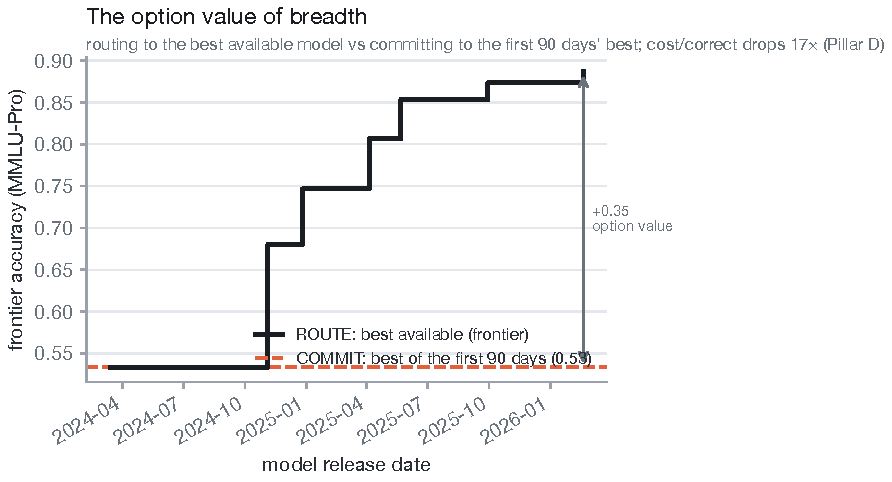
\includegraphics[width=0.55\textwidth]{figures/fig_churn.pdf}
\caption{\label{fig:churn}Optionality under churn (secondary). Frontier accuracy on MMLU-Pro over 2024--2026 (ROUTE: adopt each
new best) vs.\ committing to the best model of the window's first 90 days: a $\nChOptPro$ realized option value of breadth where headroom exists, alongside a
$\approx\!\nChDropLo$--$\nChDropHi\times$ fall in frontier dollars-per-correct.}
\end{figure}

\section{The third domain: execution-graded competitive code}\label{app:codegen}
The binding external-validity question is whether co-failure is a math artifact or tracks open-ended generation. We test it on a
\emph{structurally independent} domain, competitive programming, where generation is open-ended but grading is programmatic and
the task family is disjoint from math.

\paragraph{Construction and strict grader.} From \texttt{deepmind/code\_contests} (Codeforces rating $1900$--$3500$) we take
problems and retain only those whose \emph{own} accepted Python-3 reference our grader accepts (so the grader can accept a correct program); $63$ problems pass (of $140$ fetched; $77$ dropped, mostly for lacking a short Python-3
reference), each with a median of $20$ tests. Each model writes a stdin/stdout
program; we execute it against the problem's \emph{private} $+$ \emph{generated} stress tests (not the tiny public samples),
inside a memory-capped sandbox, enforcing $3\times$ the official (C++-calibrated) time limit---strict, but \emph{Python-fair}, so
that correct-but-slower Python is not failed (which would manufacture co-failure). $18$ models $\times$ $63$ problems
spanning rating $1900$--$3500$.

\paragraph{Result: no co-failure.} Mean accuracy is $\nCodeMeanAcc$ (these are genuinely hard problems), yet none of the
$\nCodeN$ problems is failed by every model ($95\%$ upper limit on $\beta$: $\nCodeBetaHi$). Our first release reported five
problems as a co-failure tail. Every one states that any valid answer is accepted (``if there are multiple answers, print any
of them'', or a free choice of paths or orderings), and the exact-match grader scored valid alternative outputs as wrong. We
wrote a special checker for each, as the official Codeforces judges use (\texttt{harness/code\_checkers.py}: replay the
operations, check the path or ordering, or verify the optimum), and re-ran every model's released program: each of the five
is solved by at least three models. Three of the five had also rested on Gemini-3.1-Pro calls that returned nothing and were
re-queried (App.~\ref{app:audit}). The other problems that accept several outputs are still graded by exact match, which can
only understate accuracy.

\section{Content-controlled format test: free-response GPQA (LLM-judge panel)}\label{app:opengpqa}
To test whether the science regime is an artifact of multiple choice, we hold content fixed and vary only the format: the
\emph{same} GPQA-Diamond questions, asked to $18$ frontier models without their options.

\paragraph{Question screen (version 2, protocol fixed before the new data).} Cutting a GPQA item at its first option, as our first version did,
leaves some questions unanswerable (``all the following statements are correct except'') or without a unique answer. Before
collecting any new data we fixed a protocol (\texttt{gpqa\_open\_v2/PROTOCOL.md}): every one of the $130$ questions was labelled
\textsc{keep} (self-contained, unique answer equal to the reference), \textsc{rewrite} (only the sentence that points at the
options is edited, adding no information from any option), or \textsc{exclude}, by raters who saw the question, its options and
its reference answer but never a model answer or result; a second rater, who knew the first version's results, reviewed
every label (changing none) and tagged the reason for each exclusion. The outcome was $80$
\textsc{keep}, $5$ \textsc{rewrite}, and $45$ \textsc{exclude}: $22$ because the question depends on its options and $23$ because
the reference answer is not a unique free-response answer (for instance, the silicon-abundance question whose reference value
follows only from a nonstandard reading of the bracket notation). The primary analysis uses the $85$ \textsc{keep} and
\textsc{rewrite} questions; a secondary analysis specified in the protocol drops only the $22$ option-dependent ones. Every label, rationale
and rewrite is released (\texttt{items\_v2.json}).

\paragraph{Grading by an LLM-judge panel.} Each (question, answer) is graded for equivalence to the reference by five
direct-answering judges (Claude-Sonnet-4.6, DeepSeek-V3.2, Gemini-3.5-Flash, Qwen3.7-Max, Mistral-Large-2512), majority vote,
ties counted as incorrect, and no judge grades its own model (\texttt{judge\_open\_v2.py}). Judges see each answer in full (the
first version showed them only its first 2{,}000 characters). Pairwise inter-judge agreement is $\kappa=\nKappaLo$--$\nKappaHi$
(Cohen's $\kappa$ over $10$ judge pairs). Reasoning models that exhausted the $2{,}048$-token budget and returned no answer were
re-asked at $8{,}192$ then $16{,}384$ tokens, so an empty cell is missing, not wrong.

\paragraph{Result: no co-failure tail in either format.} On the $\nOpenN$ primary questions that all $18$ models answered,
$\beta=\nOpenBeta$ ($\nOpenK$ all-wrong; $95\%$ upper bound $\nOpenBetaHi$), and multiple choice on the same questions gives
$\nOpenMcK$ of $\nOpenMcN$. Under the strictest judge rule (a correct mark needs all five judges) $\nOpenUnanK$ questions are all-wrong
($\beta\le\nOpenUnanK/\nOpenN$), and under the lenient rule $\nOpenLenK$. It is also not an artifact of dropping partially answered
questions: counting every partially answered question on which all answering models (at least $\nOpenUpMinAns$ of $18$) missed as
a co-failure gives at most $\nOpenUpK$ of $\nOpenUpN$ ($95\%$ upper bound $\nOpenUpBetaHi$). Accuracy changes little with the format
(on the $\nOpenMatchModels$ models in both runs, mean $\nOpenMcMean\!\to\!\nOpenOpenMean$, best
$\nOpenMcBest\!\to\!\nOpenOpenBest$), and the models miss different questions. The secondary analysis finds $\nOpenSecK$ all-wrong
questions of $\nOpenSecN$ ($\beta=\nOpenSecBeta$), and all $\nOpenSecFlagged$ are among the $23$ questions with a doubtful
reference answer.

\paragraph{What this changes.} Our first version reported $\beta=\nOpenOneBeta$ ($\nOpenOneK$ of $\nOpenOneN$) on free-response
GPQA and read it as decisive evidence that open-endedness, not subject matter, drives co-failure. That estimate is retired: most
of its all-wrong questions could not be answered without their options, and the judges saw truncated answers. On the primary question set, free-response
graduate science stays in the realizability-bound regime. Grading is still by an LLM panel, not human adjudication.

\section{Revision history and data audit (version 2)}\label{app:audit}
This version corrects the first release (June 2026). Its central empirical claim---a co-failure tail on open-ended
mathematics and code that pairwise $\rho$ underprices---does not survive: every mathematics question behind it traces to an
evaluation error, as does every code one (Table~\ref{tab:trace}). The theory, the certificate and the title claim stand; the measurement now supports
them for a different reason (\S\ref{sec:results}). Every change is logged in the released \texttt{DATA\_AUDIT.md} and, cell by
cell, in \texttt{rerun\_log.csv} and \texttt{regrade\_final\_report.json}; the first-release matrices are released unchanged
for comparison, and every number in this version is generated from the released data (App.~\ref{app:repro}).

\paragraph{Mathematical corrections.} (i)~Prop.~\ref{prop:cert}(iii): replacing $a_{\mathrm{sb}}$ by a confidence bound requires
a \emph{lower} bound; the first version said upper, which can wrongly certify that no policy pays, and the released certificate
tool had the same error. (ii)~Prop.~\ref{prop:cascade}: the integrated-advantage statement is now the exact identity
$\int_0^1(Q-Q_{\mathrm{mix}})\,d\gamma=a_L(1-a_L)(\mathrm{AUC}-\tfrac12)$; the first version's integrand omitted the factor
$\gamma$ and was false as stated. (iii)~The monotonicity step in the proof of Prop.~\ref{prop:poolbias} asserted a limit below
one that is in fact one; the proof is rewritten. (iv)~The optimal ensemble size in Prop.~\ref{prop:keven} is
$\lfloor k^\ast\rfloor+1$. (v)~Smaller fixes: the cascade's escalation fraction is renamed $\gamma$ to free $\beta$; the divergence is
attributed to a common-mode atom rather than to tail dependence as such; the Clayton underpricing grows slowly rather than
staying bounded.

\paragraph{Grading.} The first release's math grader compared answers without normalization and extracted \texttt{\textbackslash
boxed\{\}} with a one-level brace pattern, so correct answers failed against references written with units, variable prefixes,
thin spaces or shorthand fractions, and a reference no response could match made every model wrong at once. Its
multiple-choice extractor missed ``\textbf{Answer:} A'' and ``the final answer is: I''; its number extractor missed an answer
placed on the line after ``\#\#\#\#''; and several pillar matrices and the fusion samples had been scored by still earlier
extractors although the text said all outputs were re-graded. The corrected grader (\texttt{harness/grade.py}; the old one is
kept as \texttt{grade\_v1.py}) uses the MATH benchmark's reference answer normalization with a symbolic fallback; every released
artifact is re-scored from its raw responses. The re-scoring turned $\nMathJuneGrader$ of the $\nMathJuneK$ MATH-500 all-wrong
questions and $\nHardJuneGrader$ of the $\nHardJuneK$ on MATH-Hard into questions some model answers correctly.

\paragraph{Responses and budgets.} $\nCorruptCells$ cells held corrupt responses (no usage record, empty or cut-off content)
that had been graded wrong ($\nCorruptLlamaSmall$ of them Llama-3.2-3B); each was re-queried with the identical request
($\nCorruptRequeried$) or re-graded from a complete cached response ($\nCorruptFromCache$), as were $\nEmptyRequeried$
later-found calls that had returned no output. The truncation control, which the first version described as
applied, had only been run on an earlier matrix; it is now applied to every analysed all-wrong question. Every answer that hit its budget inside a question still failed by every
model was re-asked ($\nCappedLeft$ remain unchecked); the few re-asks that failed (most because the model is no longer served)
all sit in questions that another check resolved. The loaders' token budgets changed during the project, so the budget each run used is now
pinned explicitly (identified by grade agreement and confirmed by the cascade's samples) and recorded per cell.

\paragraph{References and questions.} Two raters who never saw the reference answer or any model output solved every question
still failed by all models; under the rule of \S\ref{sec:results}, $\nTotRefErr$ turned out to have wrong reference answers,
$\nTotAmbig$ to be ambiguous, and $\nTotGenuine$ events, on $\nTotGenuineQ$ distinct questions, to be genuine (\texttt{audit/}). Free-response GPQA was rebuilt under a
protocol written before its new data were collected (App.~\ref{app:opengpqa}).

\paragraph{Estimators and figures.} Tetrachoric correlations had been averaged over random subsets of $200$--$400$ model pairs
with unsolvable pairs clamped; every estimator is now exact or reports its Monte-Carlo error. The equal-quality figure had been
drawn from a different run than its caption described and is redrawn; the matched-quality text compared MMLU-Pro at $k{=}3$
with MATH-500 at $k{=}6$ and now compares both at $k{=}3$. Before any corrected input was used, every pillar analysis was
checked to reproduce its first-version output exactly from the first-version inputs.

\begin{table}[h]\centering\small\setlength{\tabcolsep}{5pt}
\begin{tabular}{p{5.3cm}cp{5.4cm}}
\toprule
 & version 1 (June 2026) & version 2 \\
\midrule
MATH-500 all-models-wrong rate $\beta$ & $\nMathJuneBeta$ ($\nMathJuneK/\nMathJuneN$) & $\nMathBeta$ ($\nMathK/\nMathN$; $95\%$ upper $\nMathBetaHi$) \\
MATH-Hard $\beta$ & $\nHardJuneBeta$ ($\nHardJuneK/\nHardJuneN$) & $\nHardBeta$ ($\nHardK/\nHardN$) \\
code $\beta$ & $\nCodeJuneBeta$ ($\nCodeJuneK/\nCodeJuneN$) & $\nCodeBeta$ ($\nCodeK/\nCodeN$) \\
free-response GPQA $\beta$ & $\nOpenOneBeta$ ($\nOpenOneK/\nOpenOneN$) & $\nOpenBeta$ ($\nOpenK/\nOpenN$) \\
MATH-500 best single model & $\nMathJuneSB$ & $\nMathSB$ \\
$\rho$ underprices frontier co-failure on math & $2.5\times$ & not supported (no genuine tail) \\
\bottomrule
\end{tabular}
\caption{Headline claims before and after the audit. The underpricing machinery is unchanged and applies to any
common-mode atom; the June tail it measured was an evaluation artifact (\S\ref{sec:results}, Fig.~\ref{fig:realizability}).}\label{tab:audit}
\end{table}
\end{document}
